% Use UTF-8 encoding!!
% (c) Stefan Ulbrich, 2012

\documentclass[english,ngerman]{KITreprt}

\usepackage{wrapfig}
\usepackage{float}

\addtolength{\abovecaptionskip}{-8mm}

%% -------------------------------
%% |  Information for PDF file   |
%% -------------------------------
\hypersetup{
 pdfauthor={Patrick Niklaus},
 pdftitle={Bachelor Thesis: Walking pattern generation for humanoid bipedal robots},
 pdfsubject={Not set},
 pdfkeywords={Not set}
}


%% --------------------------------
%% Obligatory Parameters:
%% --------------------------------

\renewcommand{\myname}{Patrick Niklaus}
\renewcommand{\mythesis}{\bachelorsthesis} %\mastersthesis, \bachelorsthesis, \protocol, \studienarbeit, \diplomarbeit
\renewcommand{\mytitle}{ Dynamically Stable Walking For Humanoid Bipedal Robots Based On Walking Patterns }
%\renewcommand{\myshorttitle}{Die offizielle \LaTeX-Vorlage des HIS}
\renewcommand{\myshorttitle}{}
\cfoot{\mytitle}

\renewcommand{\timestart}{1. Mai 2014}
\renewcommand{\timeend}{31. Oktober 2014}
%\renewcommand{\timeend}{\iflanguage{english}{February 7\textsuperscript{th},}{7. Februar} 2010}
\newcommand{\advisor}{Dr. Júlia Borràs Sol}
%\newcommand{\advisortwo}{Nur wenn n\"otig}

\newcommand{\clr}[2]{{\color{#1}{#2}}}
%\newcommand{\todo}[1]{\marginpar{\clr{red}{#1}}}
%\newcommand{\todo}[1]{%
%    \addcontentsline{tdo}{todo}{\protect{#1}}
%    \marginpar{\clr{red}{#1}}
%}

% Command for inserting a todo item
\newcommand{\todo}[1]{%
% Add to todo list
\addcontentsline{tdo}{todo}{\protect{#1}}%
%
\begin{tikzpicture}[remember picture, baseline=-0.75ex]%
\node [coordinate] (inText) {};
\end{tikzpicture}%
%
% Make the margin par
\marginpar{%
\begin{tikzpicture}[remember picture]%
\definecolor{orange}{rgb}{1,0.5,0}
\draw node[draw=black, fill=orange, text width = 2.5cm] (inNote)
{#1};%
\end{tikzpicture}%
}%
%
\begin{tikzpicture}[remember picture, overlay]%
\draw[draw = orange, thick]
([yshift=-0.2cm] inText)
-| ([xshift=-0.2cm] inNote.west)
-| (inNote.west);
\end{tikzpicture}%
%
}% 

\newcommand{\slpy}[1]{{\sloppy #1}}
\newcommand{\fixme}[1]{{\color{red}{FIXME: #1}}}
\newcommand{\name}[1]{\textsc{#1}}
\makeatletter \newcommand \listoftodos{\section*{Todo list} \@starttoc{tdo}}
\newcommand\l@todo[2]
    {\par\noindent \textit{#2}, \parbox{10cm}{#1}\par} \makeatother

\graphicspath{{./images/}}


\begin{document}


\selectlanguage{english}

%\selectlanguage{ngerman}


\maketitle

\tableofcontents

\chapter{Introduction}\label{introduction}

Nearly one hundred years of Sci-Fiction have established the firm image
of a mechanical humanoid servant with super human capabilities, with the
term \emph{Robot}. Today we live in a world where large parts of our
production circles are already dominated by robots. Yet, widespread
adoption of humanoid robots is still nowhere in evidence. One core
problem of humanoid robots is their inherent complexity. Vision,
cognition, manipulation and locomotion all need to be combined in one
mechanism. While every of these problems is under active research, one
has been especially resilient: Locomotion. Some robots, e.g.~the
\name{Armar III} robots, solve it by replacing the legs with a stable
base on wheels. While this yields convenient research platform, the
navigation in human environments is not as natural as for full humanoid
robots.

Over the last two decades a lot of progress has been made in humanoid
walking. Every one is familiar with the famous \name{ASIMO} robot
developed by Honda or the HRP robots developed by AIST which demonstrate
stable walking. More recently \name{ATLAS} by Boston Dynamics shows
great stability even under disturbances. Sadly most of these platforms
are closed and it is not known exactly which models are used in each
robot to derive stable walking.

As the goal for bipedal walking is to be as human-like as possible,
research on human walking is a great inspiration for robotic walking.
While the human gait can be divided into many phases, of primary
interest for the stability is the number of feet that are in contact
with the ground. For walking the ground contact alternates between both
feet and one support foot. These phases are called dual and single
support respectively. Each step starts with a dual support phase, that
shifts the center of mass to the foot that supports the weight in the
next step. The non-supporting foot (the \emph{swing foot}) is then moved
to the next foot hold. (See figure \ref{img:human-gait}) The area that
is in contact with the ground is not constant in each phase. Most
notably at the end of the single support phase the heel is lifted.
Consequently the contact changes from full sole contact to the toes.
Also the swing foot hits the ground heel first and rotate to meet the
ground while the center of mass is shifted forward.

\begin{figure*}[tb]
\vspace*{-1em}
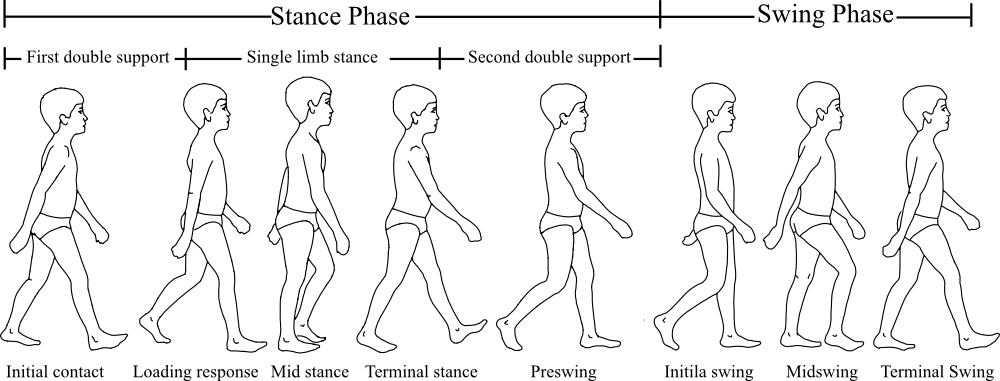
\includegraphics[width=\textwidth]{images/human_gait.png}
\caption{Phases of human gait. Source: Dynamics of Human Gait \cite{vaughan1992dynamics}, page 9}
\label{img:human-gait}
\end{figure*}

Early robots where only able to emulate this walking style to varying
degrees. A common simplification is to use a foot without movable toes.
The result is a characteristic walking style, where the foot sole is
always parallel to the ground. The most prominent example is the early
\name{ASIMO} robot. However today human-like walking using the toes has
been successfully demonstrated e.g.~by the \name{WABIAN-2R} robot
\cite{ogura2006human}.

Besides the need for an adequate kinematic structure, deriving
trajectories that are stable is not trivial. When talking about
stability, one needs to consider two cases: \emph{static} and
\emph{dynamic} stability. Static stability is concerned with the
stability of objects at rest (e.g.~standing), while dynamical stability
is concerned with the stability of objects in motion (e.g.~walking).
Deriving a stability criteria for the \emph{static} case is rather
simple. If the projection of center of mass to the ground is inside the
support polygon, the pose is said to be \emph{statically} stable. The
support polygon is the convex hull of all points of the foot that are in
contact with the ground. However dynamic stability deals with the
stability of objects (e.g.~in this case robots) in motion. In that case
more elaborate methods need to be derived using a description of the
dynamics of the robot.

There are two basic approaches to derive a trajectory for bipedal
walking. On the one side are approaches based on direct imitation of a
human motion. First a human test subject is equipped with markers. The
marker movements are recorded using motion capturing and mapped to
corresponding markers on a humanoid model. Since the kinematic structure
of a human does not map directly to the kinematic structure of a robot,
the resulting trajectory needs to be adapted to the target robot. In
general only adapting the motion based on the kinematic structure will
not yield a dynamically stable motion. Different weights and inertia
values of the links also need to be considered. However this might cause
significant modifications of the original trajectory.

On the other side there are completely synthetic approaches. Based on
simplified models of the dynamics of a humanoid robot, stability
conditions are derived. Using desired foot positions or step length and
walking speed as input, corresponding trajectories are derived that
satisfy the given stability conditions. Most notably in this category
are approaches based on the Zero Moment Point using a so called Pattern
Generator. In section \ref{section:walking-models} the ZMP is derived
for different simplified dynamic models. Fundamental for this approach
is the insight, that the dynamics of bipedal walking can be approximated
sufficiently by an inverted pendulum. The model views the center of mass
as the head of the pendulum, while the base is attached to the support
foot. Thus the task of walking can be formalized as moving the base of
the pendulum while keeping it upright.

In reality executing a trajectory that was obtained by either method is
not easy. For one, the models to approximate the dynamics of a complex
robot might be inaccurate. Also the environment the robot operates in
might not match the assumptions completely. For example a convenient
assumption is that the ground is completely flat. This is rarely the
case and needs to be controlled for. Thus a stabilizer is needed to
adapt the trajectory to the disturbances. Most stabilizer for
established robotic platforms are closed source and very robot specific.
Notably various iterations of stabilizers based on modifying an already
dynamically stable pattern where proposed by Kajita and Miura et. al.
(\cite{kajita2010biped}, \cite{miura2011human} and
\cite{kajita2012evaluation})

While a stabilizer can deal with continuous small disturbances, a robot
may encounter short but severe disturbances. These disturbances can be
viewed as pushes. Pratt et. al. established the concept of a Capture
Point, that can be used to recover from such disturbances.

This thesis presents a software framework that implements rudimentary
support for each component. They are integrated into a dynamic
simulation environment and evaluated.

\chapter{Models for humanoid walking}\label{section:walking-models}

\section{The Linear Inverted Pendulum
Model}\label{the-linear-inverted-pendulum-model}

A simple model for describing the dynamics of a bipedal robot during
single support phase is the 3D inverted pendulum. We reduce the body of
the robot to a point-mass at the center of mass and replace the support
leg by a mass-less telescopic leg which is fixed at a point on the
supporting foot. Initially this will yield non-linear equations that
will be hard to control. However by constraining the movement of the
inverted pendulum to a fixed plane, we can derive a linear dynamic
system. This model called the 3D \emph{linear} inverted pendulum model
(short \emph{3D-LIPM}).

\begin{wrapfigure}{R}{0.4\textwidth}
  \begin{center}
     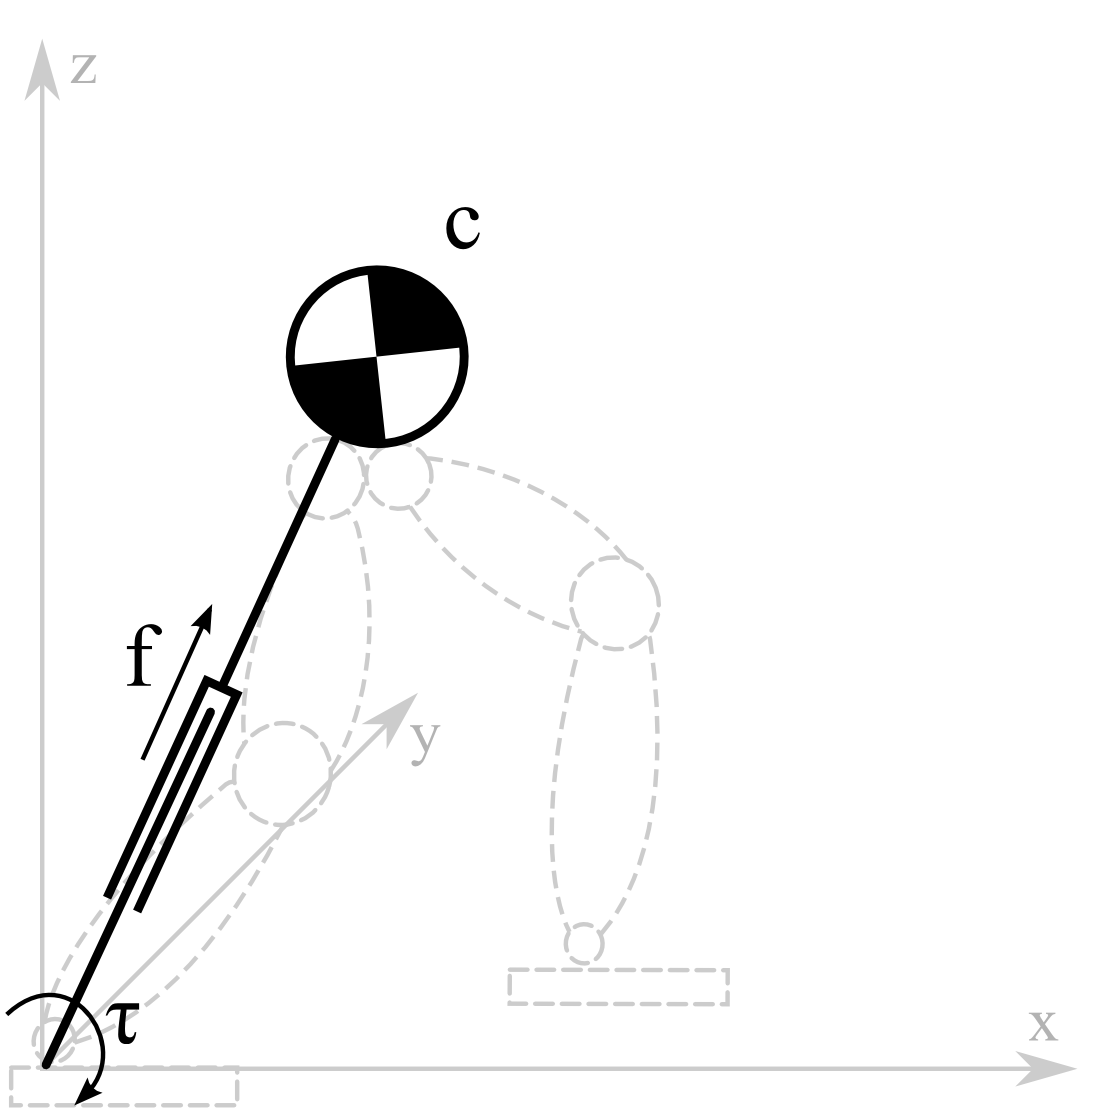
\includegraphics[width=0.4\textwidth]{images/3dlimp.png}
  \end{center}
  \caption{The 3D-LIMP}
\end{wrapfigure}

\subsection{The inverted pendulum}\label{the-inverted-pendulum}

To describe the dynamics of the inverted pendulum we are mainly
interested in the effect a given actuator torque has on the movement of
the pendulum.

For simplicity we assume that the base of the pendulum is fixed at the
origin of the current Cartesian coordinate system. Thus we can describe
the position inverted pendulum by a vector $c = (x, y, z)$. We are going
to introduce an appropriate (generalized) coordinate system
$q = (\theta_R, \theta_P, r)$ to get an easy description of our actuator
torques: Let $m$ be the mass of the pendulum and $r$ the length of the
telescopic leg. $\theta_P$ and $\theta_R$ describe the corresponding
roll and pitch angles of the pose of the pendulum.

Now we need to find a mapping between forces in the Cartesian coordinate
system and the generalized forces (the actuator torques). Let
$\Phi: \mathbb{R}^3 \longrightarrow \mathbb{R}^3, (\theta_R, \theta_P, r) \mapsto (x, y, z)$
be a function that maps the generalized coordinates to the Cartesian
coordinates. Then the Jacobian $J_\Phi = \frac{\partial p}{\partial q}$
maps the \emph{generalized velocities} to \emph{Cartesian velocites}.
Furthermore we know that the transpose $J_\Phi^T$ maps \emph{Cartesian
forces} $F = m (\ddot x, \ddot y, \ddot z)$ to \emph{generalized forces}
$(\tau_r, \tau_p, f)$.

We write $x$, $y$ and $z$ in terms of our generalized coordinates to
compute the corresponding Jacobian $J_\Phi$. From the fact that the
$\theta_P$ is the angle between the projection of $c$ onto the
$xz$-plane and $c$ and $\theta_R$ the angle between $c$ and the
projection onto the $yz$ plane we can derive the following equations
\cite{kajita20013d}:

\begin{equation}
\begin{array}{lcll} \label{eq:lip-xyz}
x & = & r \cdot \sin \theta_P & =: r \cdot s_P\\
y & = & -r \cdot \sin \theta_R & =: -r \cdot s_R \\
z & = & \sqrt{r^2 - x^2 - y^2} = r \cdot \sqrt{1 - s_P^2 - s_R^2} & \\
\end{array}
\end{equation}

From which we can compute the Jacobian by partial derivation:

\begin{equation} \label{eq:lip-Jacobian}
J = \frac{\partial p}{\partial q} = \left( \begin{array}{rcl}
0 & r \cdot c_P & s_P \\
-r \cdot c_R & 0 & s_P \\
\frac{2 \cdot r \cdot s_P c_P}{\sqrt{1 - s_P^2 - s_R^2}} & \frac{2 \cdot r \cdot s_R c_R}{\sqrt{1 - s_P^2 - s_R^2}} & \sqrt{1 - s_P^2 - s_R^2}\\
\end{array}
\right)
\end{equation}

Using the equation of motion as given by

\begin{equation}
\begin{array}{lcr}
F & = & (J^T)^{-1} \Gamma + f_g \\
m \cdot
\left(\begin{array}{c}
\ddot x \\
\ddot y \\
\ddot z \\
\end{array}\right)
& = & (J^T)^{-1}
\left(\begin{array}{c}
\tau_R \\
\tau_P \\
f \\
\end{array}\right)
+
\left(\begin{array}{c}
0 \\
0 \\
-m \cdot g \\
\end{array}\right) \\
\end{array}
\end{equation}

and equations \ref{eq:lip-Jacobian} and \ref{eq:lip-xyz} we can derive
the following equations:

\begin{equation} \label{eq:lip-dyn-y}
m(-z\ddot{y} + y\ddot{z}) = \frac{\sqrt{1 - s_P^2 - s_R^2}}{c_R} \cdot \tau_R + m g y
\end{equation}

\begin{equation} \label{eq:lip-dyn-x}
m(z\ddot{x} - x\ddot{z}) = \frac{\sqrt{1 - s_P^2 - s_R^2}}{c_P} \cdot \tau_P + m g x
\end{equation}

Observe that the terms of the left-hand side are not linear. To remove
that non-linearity we are going to use the \emph{linear} inverted
pendulum model.

\subsection{Linearization}\label{linearization}

In a man-made environment it is fair to assume that the ground a robot
will walk on can be approximate by a slightly sloped plane. In most
cases it can even assumed that there is no slope at all.

The basic assumption in the next section will be that the CoM will have
a \emph{constant displacement} with regard to our ground plane. Thus we
can constrain the movement of the CoM to a plane that is parallel to the
ground plane. Note that this assumption is, depending on the walking
speed, only approximately true for human walking as shown by Orendurff
et. al. \citep{orendurff2004effect}. For slow to fast walking ($0.7$ m/s
and $1.6$ m/s respectively) the average displacement in $z$-direction
was found to be between $2.7cm$ and $4.81$ cm. While the walking
patterns generated based on the LIP-model will guarantee dynamic
stability, they might not look natural with regard to human walking.

We are going to constrain the $z$ coordinate of our inverted pendulum to
a plane with normal vector $(k_x, k_y, -1)$ and $z$-displacement $z_c$:

\begin{equation} \label{eq:lip-z-plane}
z = k_x \cdot x + k_y \cdot y + z_c
\end{equation}

Subsequently the second derivative of $z$ can be described by:

\begin{equation} \label{eq:lip-z-div}
\ddot{z} = k_x \cdot \ddot{x} + k_y \cdot \ddot{y}
\end{equation}

Substituting \ref{eq:lip-z-plane} and \ref{eq:lip-z-div} into the
equations \ref{eq:lip-dyn-y} and \ref{eq:lip-dyn-x} yields the following
equations:

\begin{equation}
\ddot{x} = \frac{g}{z_c} x + \frac{k_y}{z_c} (x\ddot{y} - \ddot{x}y) + m z_c \cdot \tau_P \cdot \frac{\sqrt{1 - s_P^2 - s_R^2}}{c_P}
\end{equation}

\begin{equation}
\ddot{y} = \frac{g}{z_c} y - \frac{k_x}{z_c} (x\ddot{y} - \ddot{x}y) - m z_c \cdot \tau_R \cdot \frac{\sqrt{1 - s_P^2 - s_R^2}}{c_R}
\end{equation}

The term $x\ddot{y} - \ddot{x}y$ that is part of both equations is still
causing the equations to be non-linear. To make this equations linear we
will assume that our ground plane has no slope, thus $k_x = k_y = 0$ and
the non-linear terms will vanish.

Another problem is that the actuator torques $\tau_R$ and $\tau_P$ both
have non-linear factors $\frac{\sqrt{1 - s_P^2 - s_R^2}}{c_R}$ and
$\frac{\sqrt{1 - s_P^2 - s_R^2}}{c_P}$ respectively. This can be solved
by substituting with the following \emph{virtual inputs}:

\begin{equation}
\tau_R \cdot \frac{\sqrt{1 - s_P^2 - s_R^2}}{c_R} = u_R
\end{equation}

\begin{equation}
\tau_P \cdot \frac{\sqrt{1 - s_P^2 - s_R^2}}{c_P} = u_P
\end{equation}

Which yields our final description of the dynamics:

\begin{equation} \label{eq:lip-x}
\ddot{x} = \frac{g}{z_c} x + \frac{u_R}{m z_c}
\end{equation}

\begin{equation} \label{eq:lip-y}
\ddot{y} = \frac{g}{z_c} y - \frac{u_R}{m z_c}
\end{equation}

As outlined in \cite{kajita20013d} the inputs $u_P$ and $u_R$ are
generally set to zero. Thus the 3D-LIMP has no input torque. This is
desirable, as the torque that can be applied on the ankle joints is
limited. Thus it makes sense to reserve the torque for correcting
disturbances.

\section{The Zero Moment Point}\label{the-zero-moment-point}

A very popular approach to humanoid walking are schemes based on the
Zero Moment Point. One reason for that might be that it is very simple
to describe constrains for dynamic stability using this reference point.
As long as the following condition is met we will have full ground
contact of our support foot and thus can realize dynamically stable
walking: \emph{The ZMP is strictly inside the support polygon of the
support foot.}

For flat ground contact of our support foot with the floor the ZMP
corresponds with the position of the center of pressure (CoP). Indeed,
some author (notably Pratt) prefer to use the term CoP instead of ZMP.

The CoP of an object in contact with the ground can be computed as the
sum of all contact points $p_1, \dots, p_n$ weighted by the forces in
$z$-direction $f_{1z}, \dots, f_{nz}$ that is applied:

\begin{equation} \label{eq:zmp-definition}
p := \frac{\sum^N_{i=1}p_i f_{iz}}{\sum^N_{i=1} f_{iz}}
\end{equation}

An important fact (and the origin of its name) is that there are no
torques around the $x$ and $y$ axis at the ZMP:

\begin{equation}
\tau = \sum^N_{i=1} (p_i - p) \times f_i
\end{equation}

Splitting that up into each component using the definition of the cross
product yields:

\begin{equation}
\tau_x = \sum^N_{i=1} (p_{iy} - p_y) f_{iz} - \overbrace{(p_{iz} - p_z)}^{=0} f_{iy}
\end{equation}

\begin{equation}
\tau_y = \sum^N_{i=1} \overbrace{(p_{iz} - p_z)}^{=0} f_{ix} - (p_{ix} - p_x) f_{iz}
\end{equation}

\begin{equation}
\tau_z = \sum^N_{i=1} (p_{ix} - p_x) f_{iy} - (p_{iy} - p_y) f_{ix}
\end{equation}

Since we have flat ground contact, all contact points have the same
$z$-coordinate as the ZMP, thus we can simplify $\tau_x$ and $\tau_y$
to:

\begin{equation} \label{eq:zmp-torque-x}
\tau_x = \sum^N_{i=1} (p_{iy} - p_y) f_{iz} = \sum^N_{i=1} (p_{iy} f_{iz}) - (\sum^N_{i=0} f_{iz}) \cdot p_y
\end{equation}

\begin{equation}\label{eq:zmp-torque-y}
\tau_y = \sum^N_{i=1} - (p_{ix} - p_x) f_{iz} = \sum^N_{i=1} - (p_{ix} f_{iz}) + (\sum^N_{i=0} f_{iz}) \cdot p_x
\end{equation}

Furthermore we can use the corresponding components $p_x$ and $p_y$ from
the definition of the ZMP \ref{eq:zmp-definition} and substitute in the
equations \ref{eq:zmp-torque-x} and \ref{eq:zmp-torque-y}.

This will yield: $\tau_x = \tau_y = 0$.

Please note that $\tau_z$ will in general not be zero, nonetheless in
case of straight walking it is often assumed to be zero as well.

\section{The table-cart model}\label{section:table-cart}

\begin{wrapfigure}{R}{0.4\textwidth}
  \begin{center}
     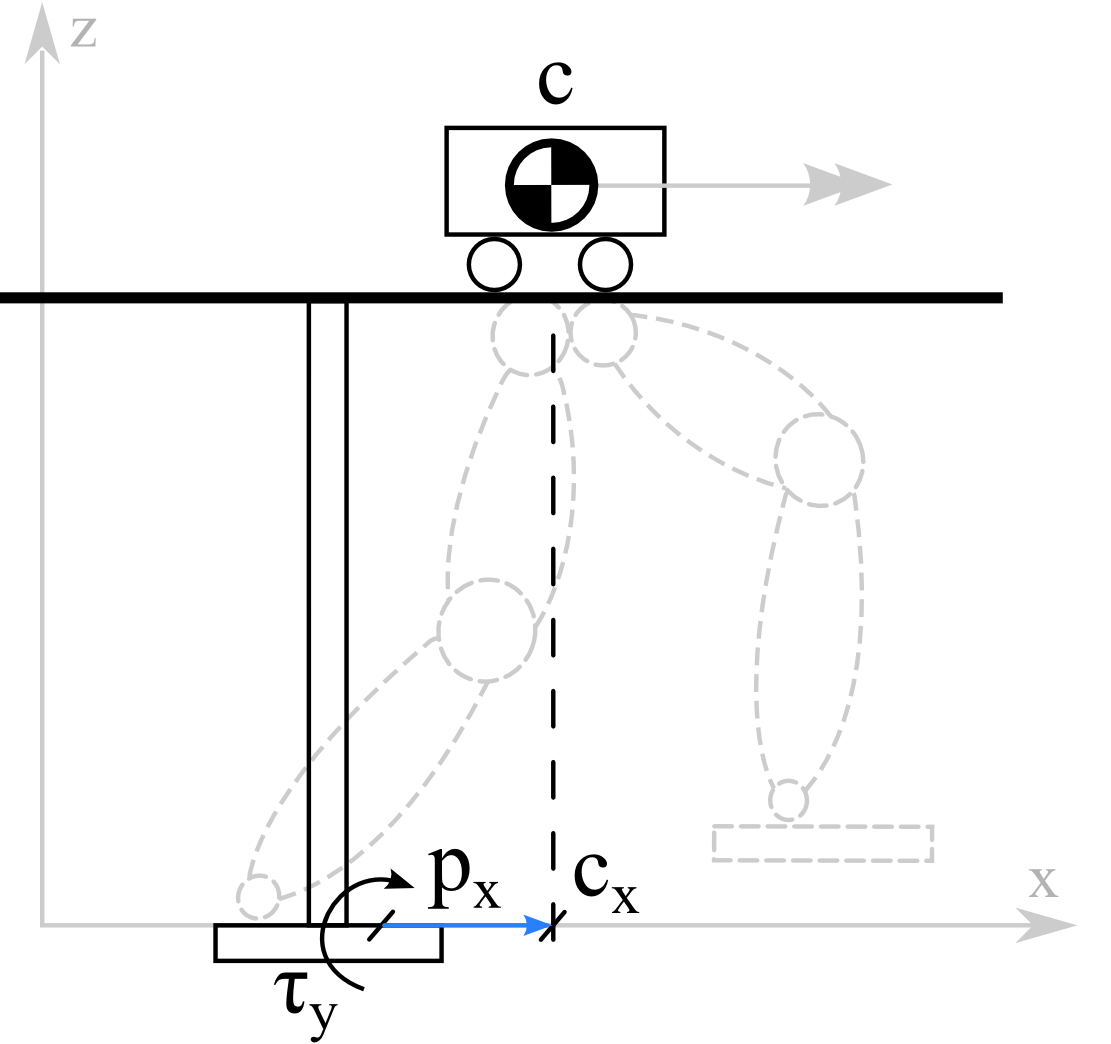
\includegraphics[width=0.4\textwidth]{images/carttable.png}
  \end{center}
  \caption{The Cart-Table model.}
\end{wrapfigure}

The table-cart model is equivalent to the 3D-LIPM model discussed
before, but somewhat more intuitive for computing the resulting ZMP from
an CoM motion. The model consists of an (infinitely) large mass-less
table of height $z_c$, while the foot of the table has the shape of the
support polygon. Given a frictionless cart with mass $m$ that moves on
the table we can compute the resulting ZMP in the support foot. Please
note that the 3D-dimensional model is equivalent to having two
independent tables with two carts each in the $xz$ and $yz$-plane
respectively. First of all, lets compute the torque $\tau_x$ and
$\tau_y$ around the x-axis and y-axis at the ZMP on the support foot.

\begin{equation}
\tau_y = \overbrace{-m g (c_x - p_x)}^{\text{torque due to gravity}} + \overbrace{m \ddot{x} \cdot z_c}^{\text{torque due to acceleration of cart}}
\end{equation}

\begin{equation}
\tau_x = -m g (c_y - p_y) + m \ddot{y} \cdot z_c
\end{equation}

Please note the similarity to the equations \ref{eq:lip-y} and
\ref{eq:lip-x} when assuming the base of the pendulum is located at $p$.
If we now use the property of the ZMP that the torque around the $x$ and
$y$-axis is zero, we can solve for the ZMP position $p$:

\begin{equation} \label{eq:zmp-x}
p_x = c_x - \frac{z_c}{g} \ddot{c_x}
\end{equation}

\begin{equation} \label{eq:zmp-y}
p_y = c_y - \frac{z_c}{g} \ddot{c_y}
\end{equation}

\section{Multi-Body methode to calculate the
ZMP}\label{section:multi-body-zmp}

Besides the simplified table-cart model, there also exists an exact
method to calculate the resulting ZMP from the movement from several
connected rigid bodies.

Let $c_i$ be the CoM position and $m_i$ the mass of the $i$-th body
($i \in \{1, ..., k\}$). Then the total linear momentum $\mathcal{P}$
can be calculated by:

\begin{equation}
\mathcal{P} = \sum^k_{j=1} m_j \cdot \dot{c}_j
\end{equation}

If $\omega_i$ the angular momentum and $R_i$ is the rotational part of
the reference frame of the $i$-th body and $I_i$ the inertia tensor in
that reference frame, the total angular momentum $\mathcal{L}$ can be
calculated by:

\begin{equation}
\mathcal{L} = \sum^k_{j=1} c_j \times (m_j \dot{c}_j) + R_j I_j R^T_j \omega_j
\end{equation}

If we denote the total mass of the robot with $M$ and the gravity vector
with $g$ we can express the change of linear momentum if a force $f$ is
applied to the body as:

\begin{equation} \label{eq:change-lin-momentum}
\dot{\mathcal{P}} = M g + f
\end{equation}

And subsequently the change in angular momentum if a torque $\tau$ is
applied:

\begin{equation} \label{eq:change-ang-momentum}
\dot{\mathcal{L}} = c \times Mg + \tau
\end{equation}

To calculate the resulting torque $\tau_{ZMP}$ around the ZMP located at
$p$ we can use:

\begin{equation} \label{eq:multi-body-zmp}
\tau_{ZMP} = \tau + (0 - p) \times f = \tau - p \times f
\end{equation}

If solve equation \ref{eq:change-lin-momentum} for $f$ and
\ref{eq:change-ang-momentum} for $\tau$ and substitute them in
\ref{eq:multi-body-zmp} this yields the following equation:

\begin{equation}
\tau_{ZMP} = \dot{\mathcal{L}} - c \times M g - p \times (\dot{\mathcal{P}} - Mg)
\end{equation}

Since we know that the torque around the ZMP is zero around the $x$ and
$y$ axis we can apply the definition of the cross product and solve for
the ZMP position:

\begin{equation}
p_x = \frac{Mgx + p_z \dot{\mathcal{P}}_x - \dot{\mathcal{L}}_y}{Mg + \dot{\mathcal{P}}_z}
\end{equation}

\begin{equation}
p_y = \frac{Mgy + p_z \dot{\mathcal{P}}_y - \dot{\mathcal{L}}_x}{Mg + \dot{\mathcal{P}}_z}
\end{equation}

Both equations are dependent on $p_z$. If we assume the robot walks on a
flat floor, we can set $p_z = 0$.

See figure \ref{zmp-comparison} to get an idea how much the Multi-Body
ZMP derives from the estimation using the Cart-Table model.

\begin{figure*}[tb]
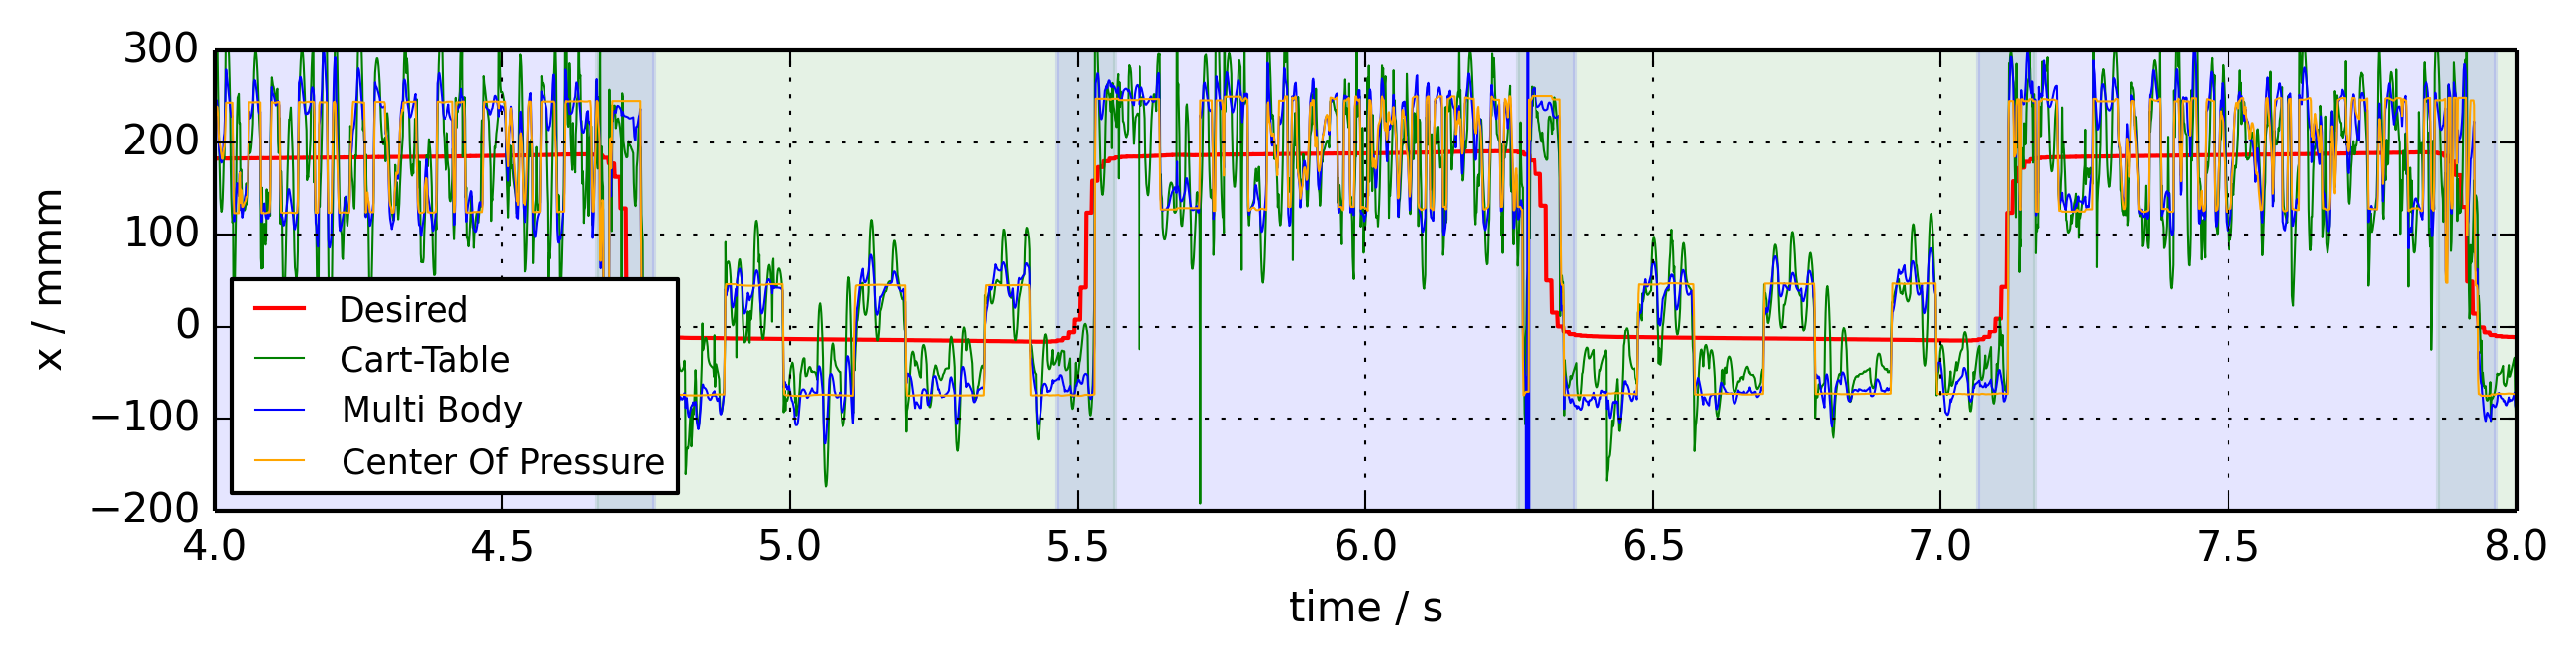
\includegraphics[width=\textwidth,resolution=300]{images/zmp_comparison.png}
\caption{Comparison of the Cart-Table and Multi-Body to estimate the realized ZMP during walking.}
\label{img:zmp-comparson}
\end{figure*}

\chapter{Pattern generator}\label{pattern-generator}

To generate a walking pattern for a bipedal robot two basic approaches
are common:

\begin{enumerate}
\def\labelenumi{\arabic{enumi}.}
\item
  Generate (or modify) foot trajectories that realize a prescribed
  trajectory of the CoM
\item
  Generate a CoM trajectory for prescribed foot trajectories
\end{enumerate}

The first approach is generally used for implementing pattern generators
solely based on the 3D-LIP model. \cite{kajita20013d} The second
approach is the more versatile one, since it is easy to incorporate
constrains of our environment (e.g.~only limited foot holds) in the
input of the pattern generator. However care must be taken while
choosing adequate step width and step length parameters for the foot
trajectory, so that they can actually be realized by the robot. The
pattern generator proposed by Kajita et al. \cite{kajita2003biped} based
on Preview Control realizes the second approach. We will discuss the
theoretical background of this pattern generator here in more detail,
since all pattern that we used where generated that way.

\section{Computing the CoM from a reference
ZMP}\label{computing-the-com-from-a-reference-zmp}

As we saw in the section \ref{section:table-cart} it is easy to compute
the resulting ZMP given the CoM and its acceleration. However for
generating the walking pattern, we want to compute the CoM trajectory
from a given ZMP. If you rearrange the equations \ref{eq:zmp-x} and
\ref{eq:zmp-y} you see that we have to solve a second order differential
equations:

\begin{equation} \label{eq:com-x}
c_x = \frac{z_c}{g} \cdot \ddot{c_x} + p_x
\end{equation}

\begin{equation} \label{eq:com-y}
c_y = \frac{z_c}{g} \cdot \ddot{c_y} + p_y
\end{equation}

There are several ways to solve this differential equations, for example
by transforming them to the frequency-domain. This however would mean,
the ZMP trajectory needs to be transformed to the frequency domain as
well, e.g.~using Fast Fourier Transformation. This has two main
problems:

\begin{enumerate}
\def\labelenumi{\arabic{enumi}.}
\item
  It has a significant computational overhead. (For FFT the additional
  runtime would be in $O(n \log n)$)
\item
  We need to know the whole ZMP trajectory in advance.
\end{enumerate}

Instead Kajita et. al. chose to define a dynamic system in the time
domain that describes the CoM movement.

\subsection{Pattern generation as dynamic
system}\label{pattern-generation-as-dynamic-system}

For simplicity we will only focus on the dynamic description of one
dimension, as the other one is analogous. To transform the equations to
a strictly proper dynamical system, we need to determine the state
vector of our system. For the table-cart model it suffices to know the
position, velocity and acceleration of the cart. Thus the state-vector
is defined as $x = (c_x, \dot{c_x}, \ddot{c_x})$. We can define the
evolution of the state vector as follows:

\begin{equation} \label{eq:dyn-system}
\frac{d}{dt} \left(\begin{array}{c}
c_x \\
\dot{c_x} \\
\ddot{c_x} \\
\end{array} \right)
=
\overbrace{
\left(\begin{array}{ccc}
0 & 1 & 0\\
0 & 0 & 1 \\
0 & 0 & 0 \\
\end{array}\right)
}^{ =: A_0}
\cdot
\left(\begin{array}{c}
c_x \\
\dot{c_x} \\
\ddot{c_x} \\
\end{array}\right)
+
\overbrace{
\left(\begin{array}{ccc}
0 & 0 & 0\\
0 & 0 & 0\\
1 & 0 & 0\\
\end{array}\right)
}^{ =: B_0}
u
\end{equation}

As you can see the jerk of the CoM was introduced as an input
$u_x = \frac{d}{dt} \ddot{c_x}$ into the dynamic system.

We use equation \ref{eq:zmp-x} to calculate the actual output of the
dynamic system the resulting ZMP, that will be controlled:

\begin{equation} \label{eq:zmp-x-output}
p_x =
\left(\begin{array}{ccc}
1 & 0 & \frac{-z_c}{g} \\
\end{array}\right)
\cdot
\left(\begin{array}{c}
c_x \\
\dot{c_x} \\
\ddot{c_x} \\
\end{array}\right)
\end{equation}

Using this formulation of the dynamic system we need to derive the
evolution of our state vector using the state-transition matrix. Since
our input ZMP trajectory will consist of discrete samples at equal time
intervals $T$ we define the discrete state as $x[k] := x(k \cdot T)$.
Please note that this system is a linear time-invariant system (LTI),
and both matrices $A_0$ and $B_0$ are constant. We can therefore use the
standard approach to solve this system using the equation:

\begin{equation}
x(t) = e^{A_0 \cdot (t - \tau)} x(\tau) + \int^t_\tau e^{A_0 \cdot (t - \lambda)} B_0 u(\lambda) d\lambda
\end{equation}

In our discrete case that becomes:

\begin{eqnarray} \label{eq:state-transition-discrete}
x[k+1] & = & e^{A_0 \cdot ((k+1)T - kT)} x[k] + \int^{(k+1)T}_{kT} e^{A_0 \cdot ((k+1)T - \lambda)} B_0 u(\lambda) d\lambda \\
       & = & e^{A_0 \cdot T} x[k] + \left(\int^{(k+1)T}_{kT} e^{A_0 \cdot ((k+1)T - \lambda)} d\lambda \right) \cdot B_0 u[k]\\
       & = & e^{A_0 \cdot T} x[k] + \left(\int^{0}_{T} e^{A_0 \cdot \lambda} d\lambda\right) \cdot B_0 u[k]
\end{eqnarray}

Keep in mind that $u(\lambda) = u[k], \lambda \in (kT, (k+1)T)$ so we
can move it outside of the integral. Let us first compute a general
solution for the matrix exponential $e^{A_0 \cdot t}$. It is easy to see
that $A_0$ is nilpotent and $A_0^3 = 0$, thus the computation simplifies
to the following:

\begin{equation}
e^{A_0 t} := \sum^{\infty}_{i=0} \frac{(A_0 \cdot t)^i}{i!} = I + A_0 \cdot t + A_0^2 \cdot \frac{t^2}{2} + 0
=
\left(\begin{array}{ccc}
1 & t & \frac{t^2}{2}\\
0 & 1 & t \\
0 & 0 & 1 \\
\end{array}\right)
\end{equation}

Using this solution computing the integral in
\ref{eq:state-transition-discrete} is quite easy:

\begin{equation}
\int^{0}_{T} e^{A_0 \cdot \lambda} d\lambda =  -\int^{T}_{0} \left(\begin{array}{ccc}1 & t & \frac{t^2}{2}\\0 & 1 & t\\ 0 & 0 & 1\end{array}\right) dt
                                            =  -\left.\left(\begin{array}{ccc} %
                                                          t & \frac{t^2}{2} & \frac{t^3}{6} \\ %
                                                          0 & t             & \frac{t^2}{2} \\ %
                                                          0 & 0             & t %
                                                 \end{array}\right)\right|_{0}^{T}\\
                                            =   \left(\begin{array}{ccc} %
                                                          T & \frac{t^2}{2} & \frac{T^3}{6} \\ %
                                                          0 & T             & \frac{T^2}{2} \\ %
                                                          0 & 0             & T %
                                                \end{array}\right)
\end{equation}

Substituting the results in \ref{eq:state-transition-discrete} yields:

\begin{eqnarray} \label{eq:state-transition-result}
x[k+1] & = &  \overbrace{\left(\begin{array}{ccc} %
                     T & \frac{t^2}{2} & \frac{T^3}{6} \\ %
                     0 & T             & \frac{T^2}{2} \\ %
                     0 & 0             & T %
               \end{array}\right)}^{=: A} x[k]
             + \overbrace{\left(\begin{array}{ccc} %
                      \frac{T^3}{6} \\ %
                      \frac{T^2}{2} \\ %
                      T %
               \end{array}\right)}^{=: B} \cdot u_x[k]
\end{eqnarray}

\subsection{Controlling the dynamic
system}\label{controlling-the-dynamic-system}

To control this dynamic system we need to determine an adequate control
input $u_x$ to realize the reference ZMP trajectory. A performance index
$J_x$ for a given control input $u_x$ is needed to formalize what a
``good'' control input would be. A naive performance index could be:

\begin{equation} \label{eq:simple-performance}
J_x[k+1] := (p^{ref}_x[k+1] - p_x[k+1])^2
\end{equation}

To minimize it, we need to find $u_x$ for which $p_x = p^{ref}_x$. By
substituting $p_x[k+1]$ with \ref{eq:zmp-x-output} and $x[k+1]$ with
\ref{eq:state-transition-result} this yields:

\begin{equation}
u_x[k] = \frac{p^{ref}_x[k+1] - C \cdot A \cdot x[k]}{C \cdot B} = \frac{p^{ref}_x[k+1] - (1, T, \frac{1}{2} T^2 -\frac{z_c}{g}) \cdot x[k]}{\frac{1}{6}T^3 - \frac{z_c}{g} T}
= \frac{p^{ref}_x[k+1] - p_x[k] - T \dot{c_x}[k] - \frac{1}{2} T^2 \ddot{c_x}[k]}{\frac{1}{6}T^3 - \frac{z_c}{g} T}
\end{equation}

To analyze the behavior of this control law for $u_x$ we simulate the
rapid change of reference ZMP when changing the support foot.

\begin{figure*}[tb]
\vspace*{-1em}
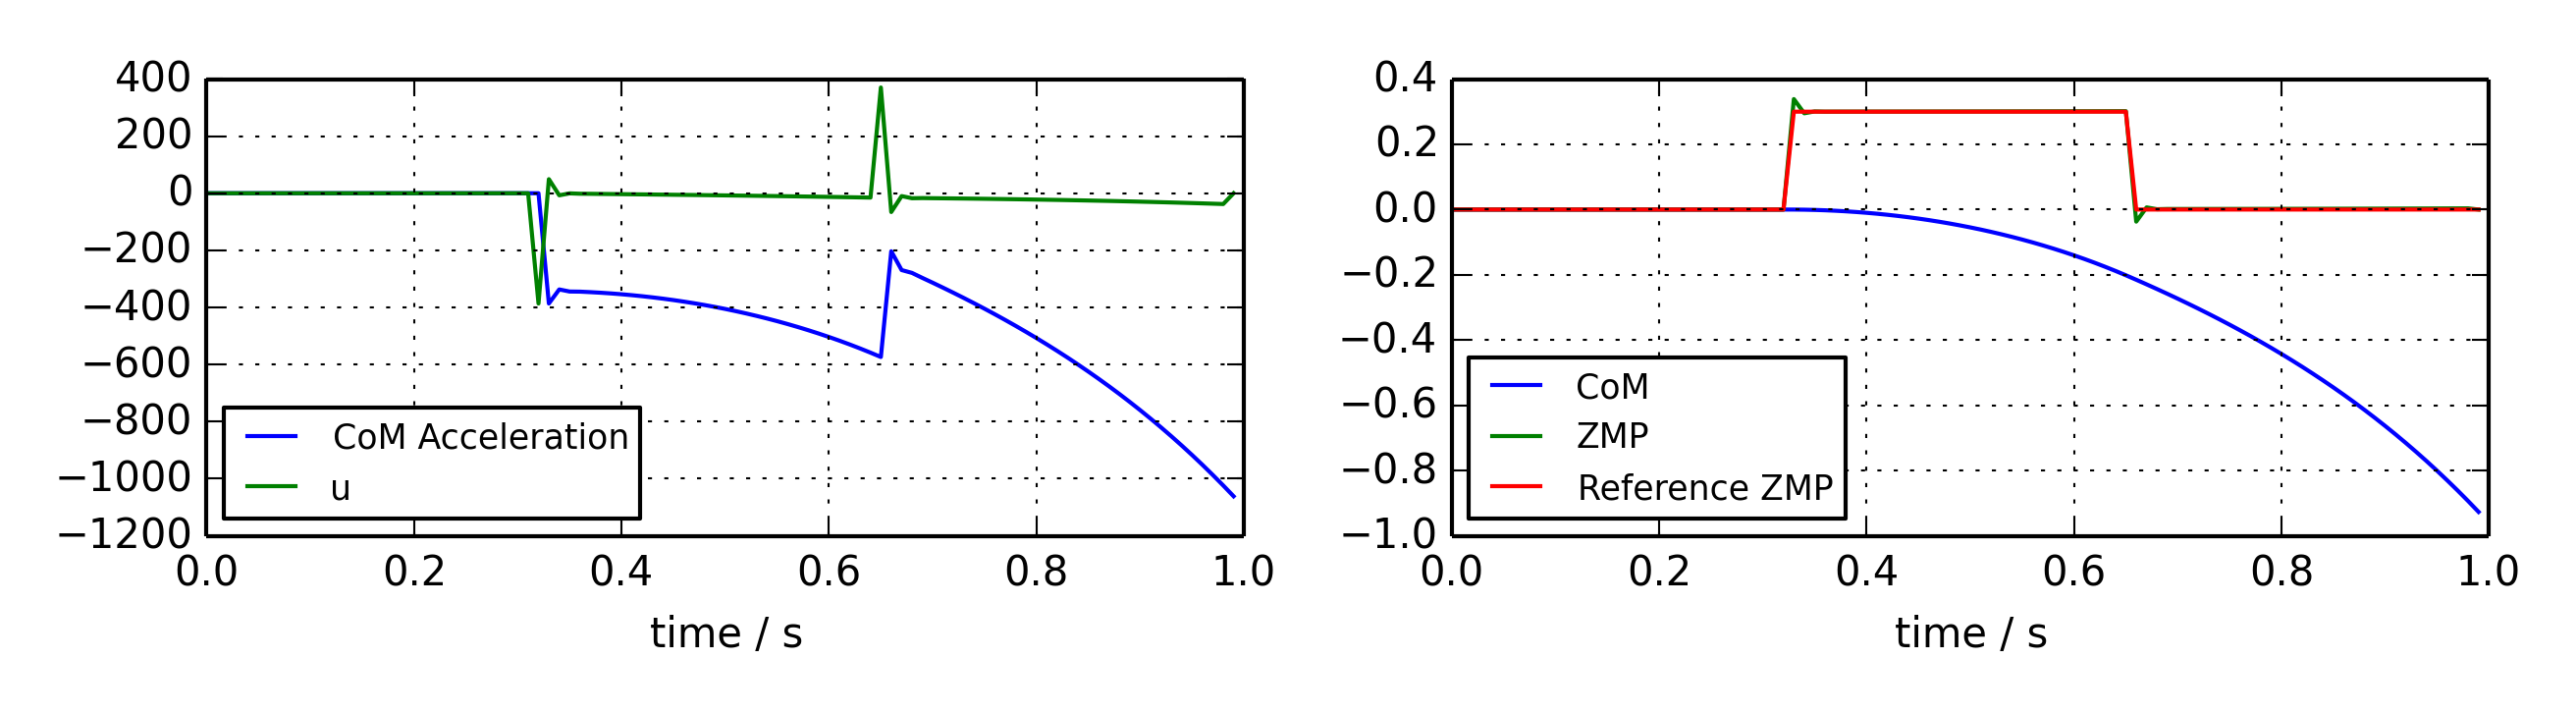
\includegraphics[width=\textwidth]{images/simple_zmp_control.png}
\caption{ZMP control based on the performance index described by equation \ref{eq:simple-performance}.}
\label{img:simple-zmp-control}
\end{figure*}

As you can see the reference ZMP is perfectly tracked. However, the CoM
does not behave as expected. To achieve the required ZMP position the
CoM will be \emph{accelerated indefinitely} in the opposite direction.
Clearly this is not desired and will lead to falling on a real robot. A
more sophisticated performance index is needed. To eventually reach a
stable state at which the CoM comes to rest, the performance index
should include a state feedback. Also note the large jerk that is
applied to the system when the reference ZMP position changes rapidly.
In a real mechanical system large jerks will lead to oscillations, which
will disturb the system. Thus the performance index should also try to
limit the applied jerk.

Another problem is caused by the very nature of a controller: The
controller starts to act \emph{after} we have a deviation from our
reference ZMP trajectory. Trying make this lag as small as possible can
lead to very high velocities, which might not be realizable by motors of
a robot. However we have at least limited knowledge of the future
reference trajectory. This knowledge can be leveraged by using Preview
Control, which considers the next $N$ time steps for computing the
performance index.

Kajita et. al. use a performance index proposed by Katayama et. al.
\cite{katayama1985design} to solve all of the problems above:

\begin{equation}
J_x[k] = \sum^{\infty}_{i=k} Q_e e[i]^2 + \Delta x[i]^T Q_x \Delta x[i] + R \Delta u_x[i]^2
\end{equation}

$Q_e$ is the error gain, $Q_x$ a symmetric non-negative definite matrix
(typically just a diagonal matrix) to weight the components of
$\Delta x[i]$ differently and $R > 0$. Conveniently Katayama also
derived an optimal controller for this performance index, which is given
by:

\begin{equation}
u[k] = -G_i \sum^k_{i=0} e[k] - G_x x[k] - \sum^N_{j=1} G_p p^{ref}_x[k + j]
\end{equation}

The gains $G_i, G_x, G_p$, can be derived from the parameters of the
performance index. Since the calculation is quite elaborate we refer to
the cited article by Katayama p.~680 for more details.

\section{Implementation}\label{implementation}

\begin{figure*}[tb]
\vspace*{-1em}
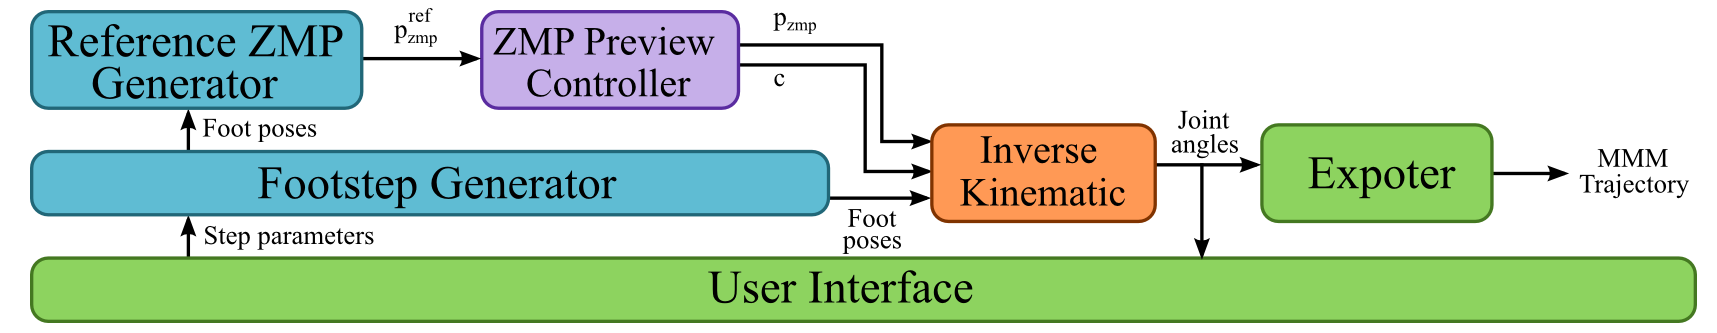
\includegraphics[width=\textwidth]{images/pattern_generator_architechture.png}
\caption{Architechture of the pattern generator}
\label{img:pattern-generator-architechture}
\end{figure*}

To generate walking patterns based on the ZMP preview control method,
the approach from Kajita was implemented in \name{libBipedal} a shared
library. A front-end was developed to easily change parameters,
visualize and subsequently export the trajectory to the \name{MMM}
format. The implementation was build on a previous implementation, which
was refactored, extended and tuned with respect to results from the
dynamics simulation.

The pattern generator makes extensive usage of
\name{Simox VirtualRobot}, for providing a model of the robot and the
associated task of computing the forward- and inverse kinematics.

Generating a walking pattern consists of multiple steps. First the foot
positions are calculated. These are used to derive the reference ZMP
trajectory which is feed into the ZMP preview controller. From that the
CoM trajectory is computed. The CoM trajectory and feet trajectories are
then used to compute the inverse kinematics. The resulting joint
trajectory is displayed in the visual front-end and can be exported.
Each step is contained in dedicated modules that can be easily replaced,
if needed. We will outline the implementation of each module separately.

\subsection{Generating foot
trajectories}\label{generating-foot-trajectories}

To generate the foot trajectories several parameters are needed:

\begin{figure*}[b]
\begin{center}
  \begin{tabular}{| l | l |}
    \hline
    $h$ & 0.1 m \\ \hline
    $l$ & 0.3 m \\ \hline
    $w$ & 0.2 m \\ \hline
    $t_{ss}$ & 0.7 s\\ \hline
    $t_{ds}$ & 0.1 s\\ \hline
  \end{tabular}
\caption{Default parameters used for generating a walking trajectory.}
\label{table:pattern-parameters}
\end{center}
\end{figure*}

\begin{description}
\item[Step height $h$]
Maximum distance between the foot sole and the floor
\item[Step length $l$]
Distance in anterior direction ($y$-Axis) between the lift-off point and
the touch-down point
\item[Step width $w$]
Distance in lateral direction ($x$-Axis) between both TCP on the feet
\item[Single support duration $t_{ss}$]
Time the weight of the robot is only support by exactly one foot
\item[Dual support duration $t_{ds}$]
Time the weight of the robot is supported by both feet
\end{description}

See figure \ref{table:pattern-generator} for the values used to generate
the trajectories using a model of the \name{Armar IV} robot.

\subsubsection{Walking straight}\label{walking-straight}

Since the foot trajectories of a humanoid walking have a cyclic nature,
we only need three different foot trajectories that can be composed to
arbitrarily long trajectories: Two transient trajectories for the first
and last step respectively and a cyclic motion that can be repeated
indefinitely. We can use the same trajectories for both feet, as they
are geometrically identical. Each foot trajectory starts with swing
phase and a resting phase. The trajectory in $y$ and $z$ direction is
computed by a 5th order polynomial that assures the velocities and
accelerations are approaching zero at the lift-off and touch-down point.
The first and last step only have half of the normal step length, since
the trajectory is starting and ending from a dual support stance, where
both feet are placed parallel to each other. Each trajectory is encoded
as a $6 \times N$ matrix, each column containing Cartesian coordinates
and roll, pitch and yaw angles.

\subsubsection{Walking on a circle}\label{walking-on-a-circle}

Much of the general structure of the foot trajectory remains the same as
for walking straight. However instead of specifying the step length, it
is implicitly given by the segment of the circle that should be
traversed and the number of steps. So extra care needs to be taken to
specify enough steps so that the generated foot positions are still.
Each foot needs to move on a circle with radius
$r_{inner} = r - \frac{w}{2}$ or $r_{outer} = r + \frac{w}{2}$ depending
which foot lies in the direction of the turn. The movement in
$z$-direction remains unaffected. However the movement in the $xy$-plane
is transformed to follow the circle for the specific foot. The same
polynomial that was previously used for the $y$-direction is now used to
compute the angle on the corresponding circle and the $x$ and $y$
coordinates are calculated accordingly. The foot orientation is computed
from the tangential (y-Axis) and normal (x-Axis) of circle the foot
follows.

\subsubsection{Balancing on one foot}\label{balancing-on-one-foot}

To test push recovery from single support stance a special pattern was
needed. To generate this another footstep planer was implemented that
generates a trajectory for standing on one foot. Starting from dual
support stance, the swing leg is moved in vertical direction until the
usual step height is achieved. Additionally the foot is moved in lateral
direction to half the step width. This reduces the necessary upper body
tilt to compensate the imbalance. For the last step the inverse movement
is performed to get back into dual support stance. This method could be
extended to walk by setting the next support foot in a straight line
before the current support foot. The swing foot would need to be moved
in an arc in lateral direction to avoid self-collisions.

\subsection{ZMP reference generation}\label{zmp-reference-generation}

As an input for the ZMP preview control, we need a reference ZMP
movement that corresponds with the foot trajectory. The reference
generator receives a list of intervals associated with the desired
support stance and foot positions as input. In single support phase, the
reference generator places the ZMP in the center of the support polygon
of the corresponding foot. Since the support polygon is convex, the
center is the point furthest away from the border of the polygon. Thus
it should guarantee a maximum of stability with regard to possible ZMP
errors. In dual support phase, the reference generator shifts the ZMP
from the previous support foot to the next support foot. Kajita et. al.
suggest using a polynomial to interpolate the ZMP positions between the
feet. However a simple step function
$\sigma(t) = \left\{\begin{array}{lr}p_1 & t \leq t_0 \\ p_2 & t > t_0 \end{array}\right.$
seems to suffice as well. Since the touch-down of the swing foot might
have a small lag, it is important that $t_0$ is the middle of the dual
support phase. This assures we do not start to move the ZMP too early.

\subsection{ZMP Preview Control}\label{zmp-preview-control}

This module implements the method described by Kajita et. al. and uses
the method outlined by Katayama et. al. to compute the optimal control
input $u[k]$. Since it is computational feasible, the preview period
consists of the full reference trajectory. For an online usage of this
method, this could be reduced to a much smaller sample size, e.g.~only
preview one step ahead. Using the system dynamics described by
\ref{eq:state-transition-result} the CoM trajectory, velocity and
acceleration can be computed. The implementation makes heavy use of
\name{Eigen}, a high performance linear algebra framework that uses SIMD
instructions to speed up calculations. Thus thus a calculation time of
6.2s could be achieved to calculate ten steps, including the inverse
kinematics.

\subsection{Inverse Kinematics}\label{inverse-kinematics}

Using the foot trajectories and CoM trajectory the actual resulting
joint angles need to be calculated. Since the kinematic model that is
used has a total of 35 degrees of freedom, we need to reduce the number
of joints that are used to a sensible value. For walking only the joints
of the legs and both the torso roll and pitch joints are used. All other
joints are constrained to static values that will not cause
self-collisions (e.g.~the arms are slightly extended and do not touch
the body). For computing the IK additional constraints where added, to
make sure the robot has a sensible pose: The chest should always have an
upright position and the pelvis should always be parallel to the floor.
To support non-straight walking, the pelvis and chest orientation should
also follow the walking direction. Thus the following method to compute
the desired chest and pelvis orientation is used:

\begin{enumerate}
\def\labelenumi{\arabic{enumi}.}
\item
  Compute walking direction $y'$ as normed mean of y-Axis of both feet:
  $y' := \frac{y_{left} + y_{right}}{|y_{left} + y_{right}|}$
\item
  Both should have an upright position $z' := (0, 0, 1)^T$
\item
  Compute $x'$ as the normal to both vectors: $x' := y' \times z'$
\item
  Pose $R'$ is given by $R' = (x', y', z')$
\end{enumerate}

A special property of the model that was used for computing the inverse
kinematics, is that TCP of the left leg was chosen as root node. Since
we can specify the root position freely, that removes the need of
solving for the left foot pose. Thus the following goals need to be
satisfied by the inverse kinematics:

\begin{enumerate}
\def\labelenumi{\arabic{enumi}.}
\item
  Chest orientation
\item
  Pelvis orientation
\item
  CoM position
\item
  Right foot pose
\end{enumerate}

A hierarchical solver was used to solve the inverse kinematics for that
goals in the given order. It was observed that specifying a good target
height for the CoM is of utmost importance for the quality of the IK.
For the model of \name{Armar IV} that used here, a height of $0.86$ m
yielded the best results.

\subsection{Trajectory Export}\label{trajectory-export}

The trajectory was exported in open \name{MMM} trajectory format. The
format was extended to export additional information useful for
debugging and controlling the generated trajectory. That means besides
the joint values and velocities the trajectory also includes the CoM and
ZMP trajectory that was used to derive them. Also information about the
current support phase is saved. For convenience the pose of chest,
pelvis, left and right foot are exported as homogeneous matrices as
well. This was done to save the additional step of computing them again
from the exported joint trajectory for the stabilizer and also eliminate
an additional error source while debugging.

\chapter{Dynamic Simulation}\label{dynamic-simulation}

To evaluate the generated trajectories a simulator for the dynamics was
developed. The simulator was build on the \name{SimDynamics} framework
that is part of \name{Simox}. \name{SimDynamics} uses
\name{Bullet Physics} as underlying physics framework. A big part of the
work on the simulator was spend on configuring the parameters and
finding flaws in the physics simulation. Thus the simulator includes a
extensive logging framework that measures all important parameters of
the simulation. For visualizing and analysing the measurement the Open
Source tools \name{IPython}, \name{numpy} and \name{pandas} where used.

\section{Simulating rigid body
dynamics}\label{section:rigid-body-simulation}

For physical simulation in general can be divided into discrete methods
and continuous methods. Discrete simulators only compute the state of
the system at specific points in time, while continuous simulators are
able to compute the state of the system at any point in time. While
continuous simulation is the more flexible approach, it quickly becomes
impractical with the number of constrains involved. Typically a large
amount of differential equations need to be solved. Since it is hard to
obtain analytical solutions for most differential equations, numerical
methods need to be used, which often have a large runtime. On contrast
discrete simulation methods only compute simulation values for specific
time steps. This exploits the observation that we will typically query
the state of the physics engine only at a fixed rate anyway, e.g.~at
each iteration of our control loop). Rather than solving the
differential equations that describe the physical system in each step, a
solution is derived from the previous simulation state.

A physical system we can typically find two kind of forces: Applied
forces and constraint forces. Applied forces are the input forces of the
system. Source of applied forces are for example objects like springs or
gravity. Constraint forces are fictional forces that arise from
constrains we impose on the system: Non-penetration constraints,
friction constraints, position constrains of joints or velocity
constrains for motors. Mathematically we can express such constrains in
the form: $C(x) = 0$ or $\dot{C}(x) = 0$ in the case of equality
constrains, or as $C(x) \geq 0$ or $\dot{C(x)} \geq 0$ in the case of
inequality constrains. For example the position constraint of a joint
$p$ connected to a base $p_0$ with distance $r_0 = ||p-p_0||$ would be:
$C(p) = || p - p_0 ||^2 - r_0^2$ If $p$ is moving with a linear velocity
$v$ a constraint force $F_c$ is applied to $p$ to maintain this
constraint. We can view $C$ as a transformation from our Cartesian space
to the constraint space. Thus by computing the Jacobian $J$ of $C$ we
can relate velocities in both spaces. Furthermore we can relate
constraint space forces $\lambda$ with Cartesian space forces using the
transpose of the Jacobian. Thus if we can find the constraint space
force $\lambda$ that is needed to maintain this constraint we can
compute $F_c$ using $F_c = J^T \lambda$. Computing this constraint space
forces is the task of the constraint solver.

The constrained solver used by \name{Bullet} and thus the constraint
solver used for simulating the patterns here is a sequential impulse
solver. To make some calculations easier, a SI solver works with
impulses and velocities rather than forces and accelerations. Impulses
and forces can be easily transformed in each other as $P = F \cdot T$
where $P$ is the impulse and $T$ the time step size. A sequential
impulse solver tries to compute the constraint force (in this case
rather impulse) $\lambda$ for each constraint \emph{separately}. For
each constraint the following steps are executed:

\begin{enumerate}
\def\labelenumi{\arabic{enumi}.}
\itemsep1pt\parskip0pt\parsep0pt
\item
  Compute the velocity that results from \emph{applied forces} on the
  body
\item
  Calculate constraint force to satisfy the velocity constraint
\item
  Compute new velocity resulting from constraint force \emph{and}
  applied force on the body
\item
  Update position of the body by integrating velocity:
  $p[n+1] = p[n] + v \cdot T$
\end{enumerate}

Of course this might not lead to a global solution, as satisfying a
constraint might violate a previously solved one. The idea is to
repeatedly loop over all constraints, so that a global solution will be
reached. Obviously the quality of this method relies on how often this
loop is executed. Consider the case of a kinematic chain where a
movement of a link always violates at least one constraint. It is clear
that this method needs a lot of iterations to yield good results in this
case. It becomes even worse in the case of a parallel kinematic that is
in contact with the ground, as is the case for a bipedal robot in dual
support stance. Solving a non-penetration constrain on either end, will
invalidate the position constraint of the next link. In turn, the
position constraint of each link needs to be updated until the other end
of the kinematic chain is reached. If the non-penetration constraint is
violated again for this end, the whole process starts again in reverse
direction. This leads to oscillations that need a lot more iterations to
level off to an acceptable level. Despite these inaccuracies using
enough solver iteration this still yields an overall usable systems.
However the velocities still will have a small random error in each
simulation step. This poses a major problem when trying to measure
accelerations, as the random error causes them to accelerate wildly.
This circumstance needs to be taken into account when dealing with
values derived from the acceleration (e.g.~the ZMP), as mean-filters
might be necessary.

\section{Practical challenges of physics
simulation}\label{practical-challenges-of-physics-simulation}

While walking only the feet of the robot are in contact with the ground.
Thus the stability of the whole robots depends on the contact of the
feet with the floor. Especially in single support phase that area is
very small with regard to the size of the robot. For that reason the
accuracy of ground contact forces and friction is of utmost importance
for the quality of the simulation. In general three classes of errors
need to be eliminated to get a good simulation:

\begin{enumerate}
\def\labelenumi{\arabic{enumi}.}
\item
  Incorrectly configured parameters, such as fictions coefficients and
  contact thresholds
\item
  Numerical errors
\item
  Inherent errors of the method
\end{enumerate}

As outline in the section about discrete time dynamic simulation, the
physics of the system are formulated as input forces and constrains that
need to be solved for the constraint forces. Since \name{Bullet} uses
the iterative approach described in section
\ref{section:rigid-body-simulation}. Thus it is important to use a
sufficient amount of iterations for each simulation step. Another
important parameter is the time step of each simulation step. Through
experimental evaluation a simulation with 2000 solver iterations and a
time step size of 1ms was sufficiently stable. However since the number
of iterations is very high and a lot of time steps are calculated during
the simulation, numeric errors become significant. That made is
necessary to enable using double precision floating point numbers for
the values used during simulation.

To decide which contact constrains are active for which points,
\name{Bullet} must solve for object collisions. Depending on the objects
involved different algorithms are used to calculate the contact points.
Major gains in accuracy could be observed by replacing the feet and the
floor with simple box shapes, instead using mesh based models.

\section{Implementation}\label{implementation-1}

\begin{figure*}[htb]
\vspace*{-1em}
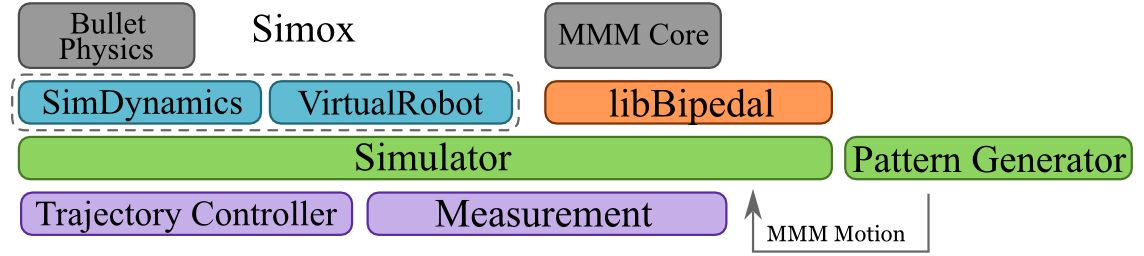
\includegraphics[width=\textwidth]{images/architechture.png}
\caption{Achitechture of the stabilizer}
\label{img:stabilitzer-achitechture}
\end{figure*}

The simulator was designed to load arbitrary motions in the \name{MMM}
format and replay them. Additional stabilization algorithms can be
applied depending on additional information provided in the \name{MMM}
motions. These stabilization algorithms are called by real-time plugins
implemented by the class \texttt{TrajectoryController}, that get invoked
in each simulation step.

Currently three controllers are implemented. A controller based on the
stabilizer proposed by Kajita (as outlined in section
\ref{section:stabilizer}), a simple heuristic stabilizer (outlined in
section \ref{section:alternative-approach}) and a controller that just
plays back the specified walking pattern. Each control algorithm is
invoked in the same cycle time as the reference walking pattern.

The resulting, possibly modified, joint angles are then interpolated
using cubic splines. This ensures a smooth velocity profile and
mitigates destabilizing oscillations caused by large velocity changes.

The interpolated angles are send via \name{SimDynamics} to the
corresponding motors. Since the motor implemented in \name{Bullet} are
velocity controlled, PID based motor controllers were added to
\name{SimDynamics}. They control the motor velocities to compensate
position errors.

The motors implemented \name{Bullet} do not limit the motor velocity and
acceleration. This is not consistent with real motors, thus limits for
velocities and acceleration where introduced to \name{SimDynamics}, that
can be configured on a per-joint basis.

\section{Simulation analysis}\label{simulation-analysis}

\begin{wrapfigure}{R}{0.6\textwidth}
  \begin{center}
     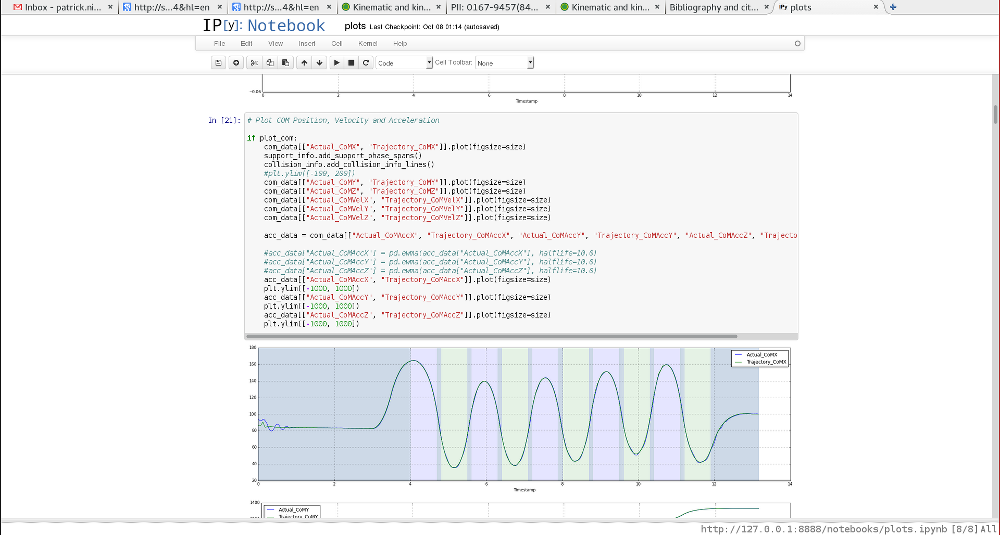
\includegraphics[width=0.6\textwidth]{images/plotting_screenshot.png}
  \end{center}
  \caption{Screenshot of ipython showing plots of the CoM obtained by a simulation}
\end{wrapfigure}

An important part of the simulation is the generation of measurements
that can be carefully evaluated offline or displayed in the
visualization. For this purpose a modular measurement component was
added to the simulator. An important design goal was to keep the
measurement component as simple to extend and maintain as possible. Each
module measures a specific set of values and writes them, indexed by the
corresponding timestamp, to its log file. As output format the well know
plain text format CSV was used. The visualization can query the
measurement components directly to get the newest values to be
displayed. For example the ZMP module measures the actual ZMP and also
provides an interface to query the trajectory ZMP and the reference ZMP
that was provided as input for the pattern generator. Thus all three
values can be displayed in the visualization and easily compared later
by analysing the log file. Since the goal was to keep the component as
simple as possible, we use existing well known tools for analyzing the
generated log files. Some small helper scripts are provided to make it
easier to load the data into the time series analysis framework
\name{pandas}. \name{Pandas} interfaces with the popular plotting
framework \name{matplotlib} to display plots of the data. \name{IPython}
is used to easily run the analysis and display the results in a browser
window. All plots of simulated patterns found in this thesis can be
generated automatically for every simulation.

\chapter{Stabilizing a trajectory}\label{stabilizing-a-trajectory}

While executing a trajectory there are several sources of errors that
will make it necessary to correct the trajectory. We can divide them in
about three main classes:

\begin{description}
\item[Disturbances of the environment:]
Pattern generator make some assumptions about the environment they
operate in. Most prominently the 3D-LIMP assumes the floor is completely
flat and has no slope. Also we assume we can navigate without colliding
with other object. Any environment that deviates from this assumption
can be seen as a disturbance.
\item[Disturbances due to simulation errors:]
Physical simulations often make a trade-off between speed and simulation
accuracy. Thus the simulation might not always behave as it was modeled
during calculating the pattern, or as it would behave in reality.
\item[Disturbances due to errors of the method:]
Often pattern generators use simplified models of the dynamics involved
to derive generation scheme. For example the pattern generator that was
used here assumes the ZMP behaves as the cart-table-model predicts.
However the real ZMP calculated from the multi-body dynamics can
substantially deviate.
\end{description}

\section{Controlling a deviation}\label{controlling-a-deviation}

When using a ZMP based control scheme to derive a walking pattern it
seems natural to check for deviations of the actual ZMP from the goal
ZMP. However a deviation from the reference ZMP does not necessarily
mean we will see any disturbance. As long as the ZMP remains inside the
support polygon the trajectory can be executed as planed. Also we saw
before, it is entirely possible to realize the reference ZMP while being
in an overall state that deviates significantly from the state we
assumed while generating the pattern. Thus we also need to check for a
deviation in the trajectory of our CoM. A common approach to correct for
CoM position is to control the pose of the chest frame of the robot.
This only works if the majority of the mass of a robot is located in the
upper body and arms. Luckily for most humanoid robots this is the case.

\section{Stabilizer}\label{section:stabilizer}

We chose a stabilizer proposed by Kajita et. al. in their 2010 paper.
\cite{kajita2010biped} The stabilizer only needs the joint trajectory of
the walking pattern augmented with a desired ZMP trajectory. This allows
the stabilizer to use patterns that where generated synthetically,
e.g.~by a pattern generator, or patterns that are the results of
(adapted) motion capturing. The method proposed by Kajita does not need
a torque controlled robot, but works with position control. This was
very important for the selection of this stabilizer. The underlying
simulation engine \name{Bullet} only supports velocity controlled
motors, consequently the torque can not be controlled directly directly.

The controller works by attaching control frames to specific points on
the robot. The reference position of this frames can be calculated from
the input trajectory using forwards kinematics. To compensate a
disturbance the orientation of a reference frame is modified. The
modified reference frames are then converted to the modified joint
angles by the inverse kinematics.

\begin{figure*}[tb]
\vspace*{-1em}
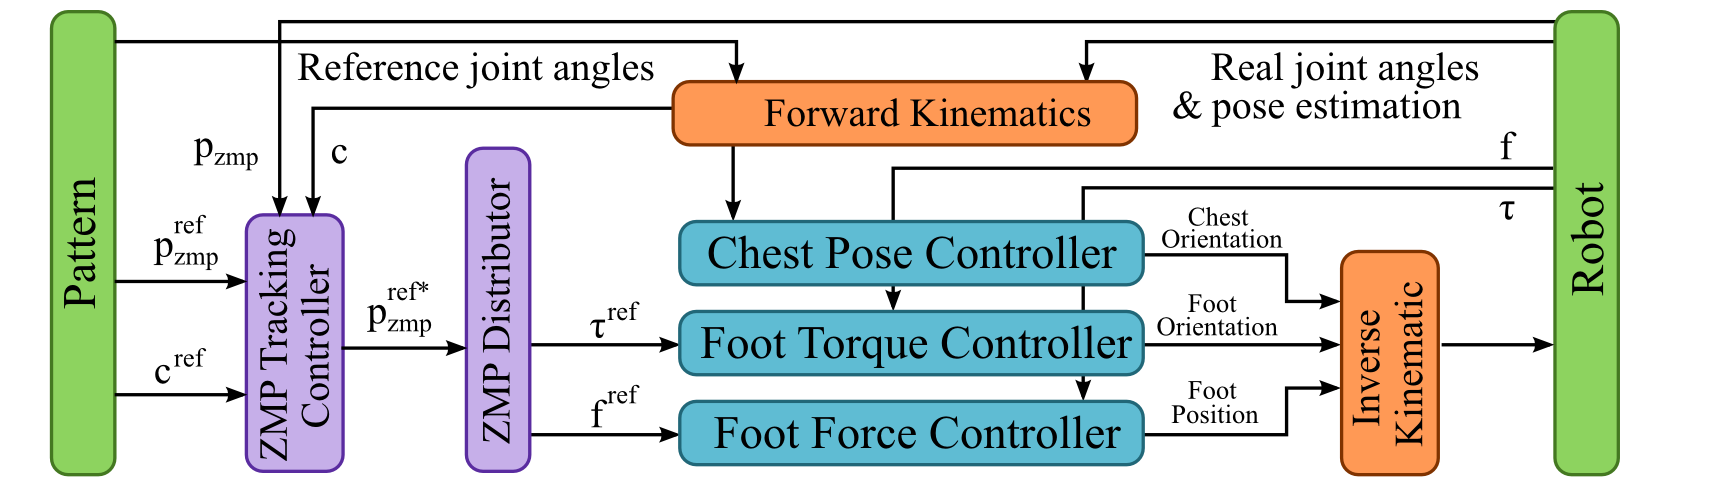
\includegraphics[width=\textwidth]{images/stabilizer_architechture.png}
\caption{Architechture of the stabilizer}
\label{img:archtitechture-stabiluzer}
\end{figure*}

In the remainder of this chapter we will use the superscript $d$ to
denote reference values and the subscript $*$ to denote modified values.

For this approach four control frames where selected. The chest to
modify the body posture, the feet to modify the ankle torque, and the
pelvis to modify the difference between contact forces of the two feet.

\subsection{Reference coordinate
system}\label{reference-coordinate-system}

\begin{wrapfigure}{R}{0.4\textwidth}
\vspace*{-1em}
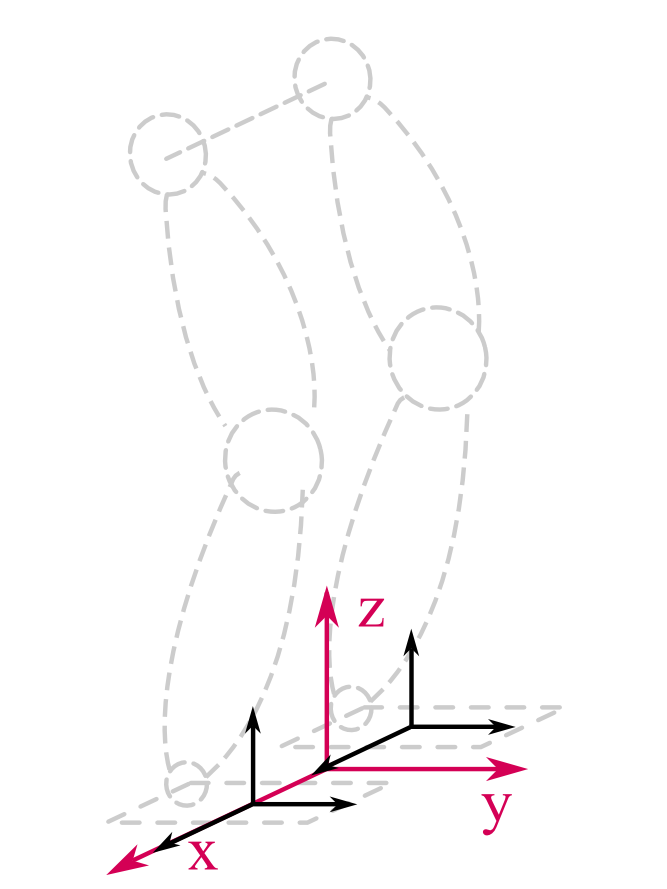
\includegraphics[width=0.4\textwidth]{images/ground_frame.png}
\caption{Ground frame in dual support}
\label{img:ground-frame}
\end{wrapfigure}

To control the ZMP and CoM it is desirable to have a reference system
that is static with respect to the ground in each support phase. It is
convenient to place the reference coordinate system in the center of the
respective support polygon. That means we place the ground frame at the
TCP of the respective foot in single support phase. As the ground frame
should be aligned with the floor, we use the projection of the foot
poses to the floor plane. In dual support phase, we calculate the pose
from the position by $p = \frac{1}{2} \cdot (p_{left} + p_{right})$ and
the $y$-axis by $y = \frac{1}{2} \cdot (y_{left} + y_{right})$. The
$z$-axis is the normal of the floor plane: $z = (0, 0, 1)$. See figure
\ref{img:ground-frame} for an example. The resulting reference frame is
called the \emph{ground frame}.

\subsection{Controlling the body
posture}\label{controlling-the-body-posture}

The control strategy of the chest pose is straight forward: Given the
reference roll angle $\phi^d$ and reference pitch angle $\theta^d$
compute the differences to the actual angles $\phi$ and $\theta$. The
main problem in a real robot is to obtain the actual global pose of this
frame. The proposed method is to use a Kalman filter to estimate the
pose from the joint position and accelerometers. We did not implement
this method in simulation, as it is easy to obtain the exact pose from
the simulator. To prevent rapid movements of the chest that cause large
accelerations, a dampening controller is used. The angles $\Delta \phi$
and $\Delta \theta$ can be calculated by the following equations:

\begin{equation} \label{eq:chest-dampening-roll}
\Delta \dot{\phi} = \frac{1}{D_c} (\phi^d - \phi) - \frac{1}{T_c} \cdot \Delta \phi
\end{equation}

\begin{equation} \label{eq:chest-dampening-pitch}
\Delta \dot{\theta} = \frac{1}{D_c} (\theta^d - \theta) - \frac{1}{T_c} \cdot \Delta \theta
\end{equation}

$D_c$ describes the dampening gain. $T_c$ is constant that describes how
long it will take to reach the normal positions $\Delta \phi = 0$ and
$\Delta \theta = 0$ respectively if there is no error.

The modified reference frame $R^{d*}_c$ can the be calculated by
rotating the reference frame by the additional angles:

\begin{equation}
R^{d*}_c = R^d \cdot R_{RPY}(\Delta \phi, \Delta \theta, 0)
\end{equation}

To get an idea how this controller compensates CoM inaccuracies consider
the case where the upper body is bent forward. Since our reference
trajectory specifies an upright upper body pose we can assume that
$\phi^d = 0$. Since the upper body is bent forward the roll angle $\phi$
will be below zero. Depending on $D_c$ we will eventually reach
$\Delta \phi \approx |\phi|$, thus the reference frame will be modified
to bent backwards to compensate the wrong pose.

\subsection{Controlling the ankle
torques}\label{controlling-the-ankle-torques}

Since the stabilizer only has the joint trajectory and desired ZMP
trajectory as input, we need a way to compute the desired actuation
torques on the ankles. The canonical way to do this, would be to solve
the inverse dynamics of the robot. However for this we need an accurate
model of the robot, including correct masses and moments of inertia for
each link. This model is not always easy to obtain and calculating the
inverse dynamics of a robot with many degrees of freedom is rather slow.
For this reason a simple heuristic is proposed to yield approximate
torques given a reference ZMP position. However in the single support
phase it is easy to calculate the \emph{exact} actuation torque on the
ankle, that is required to realize the given reference ZMP.

First we need to calculate the force in $z$-direction applied on the
foot at the ankle $p_{ankle}$ which we name $f_g$ by:

\begin{equation}
f_g = M \cdot g
\end{equation}

Where $g$ is the gravity vector and $M$ the mass of the robot. Given
$f_g$ acting on the ankle position $p_{ankle}$ we can obtain the ankle
torque in single support phase easily using the fact, that the torque
around the ZMP is zero:

\begin{equation}
\begin{array}{lcccr}
\tau_{zmp} & = & (p_{ankle} - p^d_{zmp}) \times f_g & + & \tau^d_{ankle} \\
0 & = & (p_{ankle} - p^d_{zmp}) \times f_g & + & \tau^d_{ankle} \\
\tau^d_{ankle} & = & -(p_{ankle} - p^d_{zmp}) \times f_g & & \\
\end{array}
\end{equation}

In dual support phase however that matter is more complicated. Since
both feet are in contact with the ground, the weight of the robot is
distributed between them. If we take the forces $f_R$ and $f_L$ which
act on the right ankle $p_R$ and left ankle $p_L$ respectively we know
that $f_R + f_L = f_g$. Thus there exists $\alpha \in [0, 1]$ for which:
$f_R = \alpha \cdot f_g$ and $f_L = (1-\alpha) \cdot f_g$. A heuristic
for computing this alpha is the \emph{ZMP distributor}.

The idea is to calculate the nearest points $p_{L\#}$ and $p_{R\#}$ from
the ZMP to the support polygons of the feet. If the ZMP falls inside one
of the support polygons set $\alpha = 1$ or $\alpha = 0$ respectively.
If it is outside of both support polygons the ZMP is projected onto line
from $p_{L\#}$ to $p_{R\#}$ yielding the point $p_{\alpha}$.

We can then set $\alpha$ to:

\begin{equation}
\alpha = \frac{|p_{\alpha} - p_{L\#}|}{|p_{R\#} - p_{L\#}|}
\end{equation}

If $\tau_L$ and $\tau_R$ are the torques in the left and right ankle
respectively, we can calculate the torque around the ZMP as:

\begin{equation} \label{eq:ds-torque}
\tau_{zmp} = (p_R - p^d_{zmp}) \times f_R + (p_L - p^d_{zmp}) \times f_L + \tau^d_L + \tau^d_R
\end{equation}

As before, we assume that $\tau_{zmp} = 0$ which lets us solve
\ref{eq:ds-torque} for $\tau_0 := \tau^d_L + \tau^d_R$:

\begin{equation} \label{eq:tau0-torque}
\tau_0 = (p_R - p^d_{zmp}) \times f_R + (p_L - p^d_{zmp}) \times f_L
\end{equation}

We now again apply a heuristic using the $\alpha$ computed before to
distribute $\tau_0$ to each ankle. First we need to transform $\tau_0$
from the global coordinate system to a local coordinate system described
by the \emph{ground frame}. We mark all vectors in the local coordinate
system with $'$. The heuristic applied is: The torque around the
$x$-Axis in each ankle is approximately proportional to the force
applied at that ankle. Thus:

\begin{equation} \label{eq:torque-right-x}
\tau^{d'}_{Rx} = \alpha \tau_{0x}'
\end{equation}

\begin{equation} \label{eq:torque-left-x}
\tau^{d'}_{Lx} = (1-\alpha) \tau_{0x}'
\end{equation}

The torque around the $y$-Axis depends on the direction of the total
torque $\tau_{0y}'$. If the total torque acts in clockwise direction
(negative sign), we can assume it will only be applied to the left foot.
If the torque acts in anti-clockwise direction (positive sign), we
assume it will only be applied to the right foot.

\begin{equation} \label{eq:torque-right-x}
\tau^{d'}_{Ry} = \left\{
\begin{array}{lr}
\tau_{0y}', & \tau_{0y'} > 0 \\
0, & else
\end{array}
\right.
\end{equation}

\begin{equation} \label{eq:torque-left-x}
\tau^{d'}_{Ly} = \left\{
\begin{array}{lr}
\tau_{0y}', & \tau_{0y'} < 0 \\
0, & else
\end{array}
\right.
\end{equation}

We can now transform the torques form our local coordinate system to the
coordinate system of the corresponding foot yielding $\tau^d_L$ and
$\tau^d_R$.

Now that we have obtained the reference torques, we can try to control
the torque in each angle using the measured torques $\tau_R$ and
$\tau_L$. However since we assume a position controlled robot, the
torque differences need to be translated into pose changes. There are
three primary cases that need to be considered if we change the
reference pose of a foot:

\begin{description}
\item[The foot is not in contact with the ground:]
Changing the reference pose will just affect the foot
\item[The foot is in contact with the ground, but the contact is
non-solid:]
If the foot has a soft contact surface (e.g.~rubber) we can model the
contact with the ground as springs that connect the ground with the
contact points on the foot. Changing the pose of the foot will
relax/compress the springs and change the contact forces accordingly.
\item[The foot is in solid contact with the ground:]
Changing the reference foot pose \emph{will not change the foot pose at
all}. Instead, the pose of the rest of the robot is changed. If the foot
pose is changed by the angles $\Delta \phi$ and $\Delta \theta$ all
other frames of the robot will be changed by $-\Delta \phi$ and
$-\Delta \theta$.
\end{description}

For a foot with a rubber surface we will start with a non-solid contact
and transition to a solid contact, once the rubber is sufficiently
compressed. \cite{kajita2005running}

To get an idea how changing the pose on such a foot with rubber surface
affects the torque, consider the case of rotating the foot around its
lateral axis ($x$-Axis) in anti-clockwise direction. Since the contact
with the ground is at first non-solid, we can employ the spring model.
The springs at the front of the foot are compressed thus the force
applied at the corresponding contact points increases. Accordingly the
springs at the back are compressed less, thus the force applied to the
corresponding contact points decreases. Resulting we see a increase in
torque around the $x$-axis.

If the springs are compressed sufficiently, we can assume the contact
with the floor is solid. Since the pose of the foot does not change, the
increase in the joint angle in the ankle will rotate the upper body
backwards. Recall the 3D-LIMP model for a moment, in that model this
means our pendulum swings backwards. This will lead to an increase of
the torque around the $x$-Axis in the base of the pendulum, the ankle
joint.

For rotating the foot around the $y$-axis the same ideas hold. As a
result we see that additional foot rotation long the $x$- and $y$-Axis
have a proportional relationship with the torque around that axis. This
motivates the definition of the controller proposed by Kajita et. al.
The additional rotation angles are can be calculated by the following
equations:

\begin{equation}
\Delta \dot{\phi_i} = \frac{1}{D_{ix}} (\tau^d_{ix} - \tau_{ix}) - \frac{1}{T_{ix}} \cdot \Delta \phi_i
\end{equation}

\begin{equation}
\Delta \dot{\theta_i} = \frac{1}{D_{ix}} (\tau^d_{iy} - \tau_{iy}) - \frac{1}{T_{ix}} \cdot \Delta \theta_i
\end{equation}

Where $i \in \{R, L\}$. This again utilizes the same concept of a
dampening controller that was used previously for controlling the chest
frame orientation. We can use the obtained angles $\Delta \phi_i$ and
$\Delta \theta_i$ to compute the modified reference frames for the feet:

\begin{equation}
R^{d*}_i = R^d_i \cdot R_{RPY}(\Delta \phi_i, \Delta \theta_i, 0)
\end{equation}

\subsection{Foot force difference
controller}\label{foot-force-difference-controller}

In the previous section only the ankle torque were controlled to match
the reference values that were derived using the ZMP distributer.
However reference values for the gravitational force that each foot
exerts on the ground were also obtained. These forces are not
necessarily realized. Consider the case of slightly uneven ground. If
the pattern assumed a flat ground, the ankle of both feet will have the
same altitude. Depending on variation of floor height, that might lead
to one foot not touching the ground at all. In the case of feet with
rubber soles, slight variations in floor height lead to a different
compression of the soles. Both cases cause a different force acting on
each foot.

If we assume the mass $M$ of the robot and the gravity vector $g$ are
correct, we know that the reference force $f^d_g = M \cdot g$ will
exactly match the force in $z$-direction $f_g$ exerted by the support
foot in single support. Thus in single support we can guarantee that we
realize our reference force. In dual support we know that
$f^d_L + f^d_R = M \cdot g$. If we apply the same reasoning as above we
know that $f^d_L + f^d_R = f_L + f_R$. If we can additionally make sure
that $f^d_L - f^d_R = f_L - f_R$ we can deduce that $f^d_L = f_L$ and
$f^d_R = f_R$. Equation \ref{eq:ds-torque} can be used to calculate the
ZMP position from the applied forces and torques on the foot. If both
reference torques and reference forces on the feet are realized, that
will guarantee the reference ZMP is also realized.

Since the $x$ and $y$ components of both $f^d_L - f^d_R$ and $f_L = f_R$
are zero we only need to control the $z$ components. As we motivated in
the beginning of this section, differences in floor height are the main
cause of deviation in the force. To compensate that, the height of the
ankle needs to be changed. Thus the difference in ankle height $z_{ctl}$
was chosen to compensate the difference in forces exerted by the foot.
The description of the controller again uses the concept of a dampening
controller, that was used in the previous sections.

\begin{equation}
\dot{z}_{ctl} = \frac{1}{D_z} [(f^d_L - f^d_R) - (f_L - f_R)] - \frac{1}{T_z} z_{ctl}
\end{equation}

Two methods were proposed to realize this difference in ankle height.
The first method is straight forward change the reference position of
the feet in $z$-direction:

\begin{equation}
p^{d*}_R = p^d_R + 0.5 \cdot \left(\begin{array}{c}0 \\ 0 \\ z_{ctl} \end{array}\right)
\end{equation}

\begin{equation}
p^{d*}_L = p^d_L - 0.5 \left(\begin{array}{c}0 \\ 0 \\ z_{ctl} \end{array}\right)
\end{equation}

This can lead to singularities if both legs are already fully stretched,
as the edge of their workspace is reached. The second method relies on
an additional rotating the pelvis link. For this approach to work, the
robot needs a joint that allows rotations around the anterior axis
($y$-Axis) to keep the upper body upright. Since the robot model we used
does not have this DOF, we only implemented the first approach.

\subsection{Interaction between
controllers}\label{interaction-between-controllers}

While each controller operate independently, their effects are highly
coupled. The most important coupling exists between the chest posture
controller and the ankle torque controller. Recall that in case of a
solid contact with the ground the ankle torque controller will not
rotate the supporting foot but rather the body of the robot. This will
however change the posture of chest frame. The chest posture controller
compensates that and keeps the body upright. This tight coupling makes
tuning the parameters $D_i$ and $T_i$ of the controllers difficult, as
their performance depends on the other controllers. Best results where
observed when the chest posture controller was tuned independently
first, disabling the other controllers. Then the foot force controllers
was enabled and tuned and finally the ankle torque controller was added
and tuned.

\subsection{CoM and ZMP control}\label{com-and-zmp-control}

The controllers specified in the previous sections can make sure, that
the ZMP that is realized tracks the ZMP that would result from a perfect
execution of the input pattern. However depending on how the reference
ZMP was predicted, that prediction might have already been wrong. For
example the ZMP Preview Control approach uses the Table-Cart model to
predict the ZMP. That prediction can deviate significantly from the real
ZMP as the model simplifies the dynamics. Thus to make sure the desired
ZMP is tracked accurately, the reference ZMP needs to be adapted as
well.

Kajita et. al. propose a dynamic system that describes the 3D-LIMP
dynamics. To model mechanical lag they introduce a parameter $T_p$ that
should specify the ZMP delay. The state-space description of the dynamic
system for the $x$-direction is given below. As before, the description
of the dynamic system for the $y$-direction is analogous.

\begin{equation} \label{eq:dyn-system-adaption}
\frac{d}{dt} \left(\begin{array}{c}
c_x \\
\dot{c}_x \\
p_{zmp_x} \\
\end{array} \right)
=
\overbrace{
\left(\begin{array}{ccc}
0 & 1 & 0\\
\frac{g}{z_c} & 0 & -\frac{g}{z_c} \\
0 & 0 & -\frac{1}{T_p} \\
\end{array}\right)
}^{ =: A}
\cdot
\left(\begin{array}{c}
c_x \\
\dot{c}_x \\
p_{zmp_x} \\
\end{array}\right)
+
\overbrace{
\left(\begin{array}{c}
0 \\
0 \\
\frac{1}{T_p} \\
\end{array}\right)
}^{ =: B}
u
\end{equation}

As controller a feedback controller is proposed:

\begin{equation}
p^{d*}_x = u = (k_1, k_2, k_3) \cdot
\left[
\left(\begin{array}{c}
c^d_x \\
\dot{c}^d_x \\
p^d_{zmp_x} \\
\end{array}\right)
-
\left(\begin{array}{c}
c_x \\
\dot{c_x} \\
p_{zmp_x} \\
\end{array}\right)
\right]
+ p^d_{zmp_x}
\end{equation}

To derive the corresponding gains $(k_1, k_2, k_3)$ pole-placement with
the poles $(-13, -3, \sqrt{\frac{g}{c_z}})$ was proposed. The gains can
be easily computed from the poles, $A$ and $B$ using predefined
functions in \name{MATLAB} or similar software.

\section{Implementation}\label{implementation-2}

To implement the stabilizer above, a number of problems had to be
solved. For one, computing the inverse kinematics is challenging. During
walking the base of support depends on which foot is in contact with the
ground. For example, if the left foot is the support foot, it is
considered the base and the right foot is considered the TCP. The
reverse is true if the right foot is the support foot. In dual support
phase, we actually have two bases of support, which yields a parallel
kinematic chain. \name{Simox}, the framework used to compute the inverse
kinematics, describes the kinematic structure of a robot as a directed
tree. Solving the inverse kinematics was initially only possible for
sub-trees of that tree. Which means it was not possible to chose base
and TCP freely, but it was determined by the structure in which the
kinematic model was initially described.

As a first approximation, a kinematic model with the left foot as root
node was used. In the case of the right foot being the support foot,
this approach leads to an increased error. Consider solving the inverse
kinematics for both legs using a differential solver in two steps: First
from the base (the left foot) to the pelvis, then from the pelvis to the
right foot. Lets assume the IK computes a perfect solution to place the
pelvis link and only achieves a small pose error of $e_{\alpha} = 0.1°$
in the pitch angle of the right foot. If the trajectory is execute, the
right foot will achieve its target pose, since it is constrained by the
ground contact. However the error in the right foot pose will effect all
other frames of the robot. Assuming a offset of $v = (-0.5, 0, 1)^T m$
from the right foot to the pelvis link, we can compute the realized
pelvis offset as
$v' = R_y(-e_{\alpha}) \cdot v = (-0.49825, 0,  1.00087)^T m$ Which
yields $1.76mm$ error in x-direction and $0.87mm$ error in y-direction.

To solve this \name{Simox} was extended by a function
\texttt{cloneInversed} that can compute a kinematic structure with
arbitrary root placement from an existing description. For the parallel
kinematic chain, it proofed sufficient to approximate it as a normal
kinematic chain and constrain the base and TCP targets accordingly.
However since the position of one foot will have small positioning
errors, there will be some jitter introduced into the system.
Integrating a solver for parallel kinematics might decrease some of the
jitter observed in foot contact forces during dual support, as the
constraint solver used for the simulation will only amplify this jitter.

As was the case with the components of the pattern generator, the core
of the stabilizer is implemented as part of \name{libBipedal}. A plugin
integrates the stabilizer into the dynamic simulation.

\section{Problems}\label{problems}

Some problems became immediately clear when testing the stabilizer
proposed by Kajita. The ground reaction forces in dual support are
oscillating wildly. Instead of a continuous force at about
$0.5 \cdot f_g$ the forces on both feet oscillate between $0$ and $f_g$,
the support foot changes in rapid successions. As outlines in section
\ref{section:rigid-body-simulation} this is a result of the constraint
solver method employed by \name{Bullet}. Subsequently the measured
torques on the ankles did not follow the prediction as well. Please note
that this is not merely sensor noise, these are the actual values used
by the simulator. Even when adding mean-filters to smoothen the measured
torques it was not possible to extract a meaningful control signal.
Besides the sequential impulse solver newer versions of \name{Bullet}
support a solver based on the Featherstone algorithm. Given the scope of
this thesis, integrating that solver was out of question, thus an
alternative approach to stabilizing had to be found.

\section{Alternative approach}\label{section:alternative-approach}

A simple heuristic, we used the controllers proposed by Kajita as
inspiration and replaced the force and torque feedback with the pose
error of pelvis and feet frames respectively. The chest controller
(Equation \ref{eq:chest-dampening-roll} and
\ref{eq:chest-dampening-pitch}) Kajita et. al. proposed for controlling
the body posture where adapted to all control frames to provide a
feedback on the pose error.

This yields a controller that keeps the feet pose parallel to the
ground, which is important when the swing foot touches the ground.
Controlling the pelvis and chest pose to follow the reference also keeps
the robot upright. It should be noted that it is not feasible to
implement this stabilizer in practice. As mentioned in section
\ref{section:stabilizer} precisely estimating the pose of a robot is not
easy. While the dampening controllers can be configured to smoothen a
noisy sensor signal, a high level of precision is required to ensure a
correct foot posture.

Since the ZMP and CoM trajectory is not adapted, the compensation of
environment disturbances is only based on a fast controller reaction to
leave the reference trajectory as little as possible and the stability
margins the ZMP provides. However as we will discuss in the evaluation
section, this simple approach is already surprisingly resilient.

\chapter{Push recovery}\label{push-recovery}

As we saw in the chapter about Stabilizers, not all disturbances can be
compensated. If the disturbance reaches a certain severity, the
trajectory can not be executed as planed without falling. Thus the
trajectory needs to be changed radically to avoid falling. There is
little hope to recover from continuous heavy disturbances, as any
attempt to recover will be defeated. Thus we focus on short but severe
disturbances, pushes.

The most prominent method to recover from pushes is the Capture Point.
The idea is to find a point, that will guarantee that the CoM comes to a
rest, if the support foot is instantaneously placed there. The push
recovery implemented here uses a simplistic method based on the Capture
Point.

\section{Capture Point}\label{capture-point}

Koolen et. al. \cite{koolen2012capturability} derive the Capture Point
for multiple models based on the 3D-LIPM. The simplest model is the 3D
Linear Inverted Pendulum with a point contact and a massless telescopic
rod. If we use the LIP equations \ref{eq:lip-x} and \ref{eq:lip-y} with
zero input torque, we can derive that so called \emph{orbital energy} of
the pendulum. As we did in the section about the pattern generator, we
will derive the equations only for one dimension. The other dimension
follows analogous.

The base of the pendulum is assumed to be at the origin of the reference
frame in \ref{eq:lip-x}. Since we want to specify the location freely,
we need to substitute $x$ with $x - p$ to yield:

\begin{equation} \label{eq:lip-x-general}
\ddot{x} = \frac{g}{z_c} (x - p)
\end{equation}

The orbital energy $E_x$ can be derived by integrating
\ref{eq:lip-x-general}:

\begin{equation} \label{eq:orbital-x}
E_x = \frac{1}{2} \dot{x}^2 - \frac{g}{2 \cdot z_c} (x - p)^2
\end{equation}

For the CoM to come to a rest the orbital energy $E_x$ must be zero.
Thus we can solve \ref{eq:orbital-x} to yield the point $p$ that will
achieve this. Since it is a quadratic equation there are two solutions:

\begin{equation}
p = x - \sqrt{\frac{z_c}{g}} \dot{x} \:\:\:\:\text{ or }\:\:\:\: p = x + \sqrt{\frac{z_c}{g}} \dot{x}
\end{equation}

Since it is generally desirable to chose a point that lies in the
direction of the CoM motion we define the \emph{Immediate Capture Point}
as:

\begin{equation} \label{eq:icp}
p_{ic} := x + \sqrt{\frac{z_c}{g}} \dot{x}
\end{equation}

Placing the base of the pendulum (the ankle) there
\emph{instantaneously} will cause an orbital energy of zero, thus the
head of the pendulum (the CoM) will stop at $p_{ic}$. In most cases we
will not be able to move the base of the pendulum instantaneously. So we
are more interested in the Immediate Capture Point in $\Delta t$ seconds
from now. This point can be obtained by \ref{eq:future-icp}. For a
detailed derivation, we recommend the paper by Koolen et. al.
\cite{koolen2012capturability}.

\begin{equation} \label{eq:future-icp}
p_{ic}(\Delta t) = p_{ankle} + (p_{ic}(0) - p_{ankle}) \cdot e^{\frac{g}{z_c} \cdot \Delta t}
\end{equation}

Where $p_{ankle}$ is the current position of ankle of the support foot
(the current base of the pendulum). and $p_{ic}(0)$ is the current
Immediate Capture Point as calculated by equation \ref{eq:icp}.

\section{Fall detection}\label{fall-detection}

The first important step to recover from a large disturbance is to
detect it. That means we need to detect if we reached a unstable state,
from which it is unlikely that we can recover only by means of the
stabilizer. We can use the measured ZMP to obtain a heuristic for such
states. If the ZMP is outside or on the edge of the support polygon, the
Cart-Table model does not guarantee stability. However in normal
operations it is likely that the ZMP will touch (or leave) the border of
the support polygon for short periods of time. A simple method to filter
out this noise is to define a minimum duration the ZMP as to be in an
unstable state. Choosing a small value will let us react faster to
disturbances, but make the method error prone. Choosing a large value
will add an additional detail until we can react, but is much less prone
to be triggered by mistake. An experimental evaluation yielded good
results with a duration of $t = $ \fixme{add real time here}.

\section{Recovery}\label{recovery}

If a fall is detected, a recovery maneuver needs to be executed. In
single support phase, that means we need to place the swing foot at the
capture point. In dual support phase we try to move the support foot
that is closest to the capture point. Recall that the base of the
pendulum coincides with the ZMP in our model view. Thus if the resulting
support polygon includes the capture point, the position will be stable.
Since the motor velocities are limited, we need a minimal amount of time
$t_{min}$ to place the foot in the desired location. Thus instead of
using the Immediate Capture Point, we use the future Immediate Capture
Point $p_{ic}(t_{min})$ to derive the desired location.

\section{Implementation}\label{implementation-3}

The stabilizer that is outlined in chapter \ref{section:stabilizer} was
extended to call the fall detection module in each iteration of the
control loop. If an unstable state is reached, the recovery module
overrides the normal trajectory of the stabilizer. After completing the
recovery maneuver, the robot remains in the given position. Resuming the
original pattern requires planning dynamically stable transition
trajectory. This is left for future work.

\chapter{Results}\label{results}

To test the performance of the stabilizer against simple pattern
playback, both walking straight and walking in circle where tested. To
simulate further disturbances, the simulation shoots a football at the
robot. In the unstabilized case, only the joint trajectory that is
generated by the pattern generator is interpolated and replayed. In the
stabilized case the alternative stabilizer described in section
\ref{section:alternative-approach} is used.

\section{Undisturbed walking}\label{undisturbed-walking}

\subsection{Walking in a straight
line}\label{walking-in-a-straight-line}

The first scenario is walking in a straight line for 10 steps. Figure
\ref{img:player-undisturbed-straight-thumbs} shows the simulation of
walking straight for 10 steps using no stabilization.

\begin{figure}[H]
\vspace*{-1em}
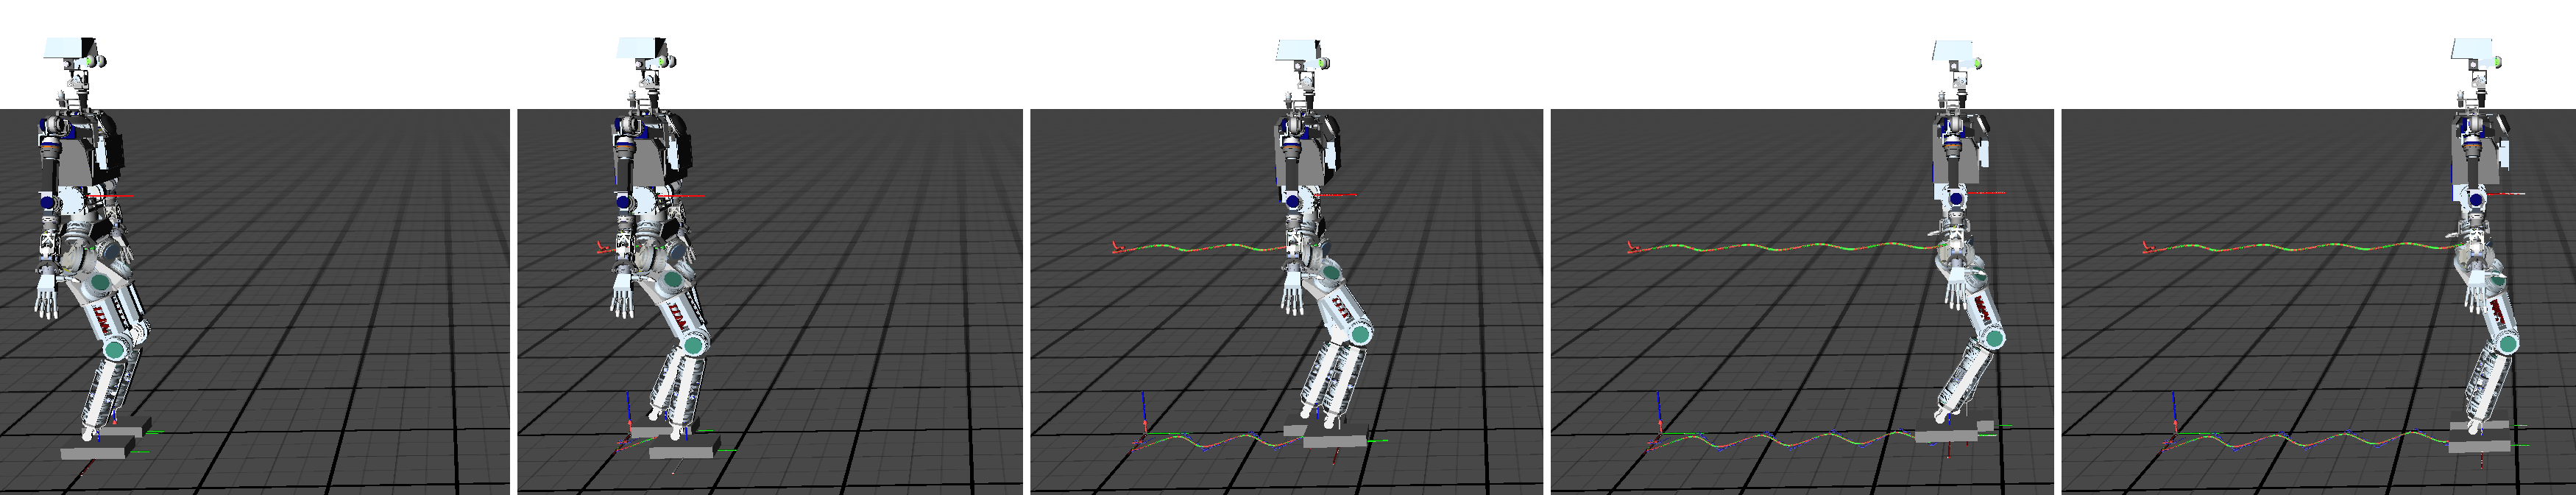
\includegraphics[width=\textwidth]{images/undisturbed_straight_thumbs.png}
\caption{Frames of undisturbed straight walking}
\label{img:player-undisturbed-straight-thumbs}
\end{figure}

\begin{figure}[H]
\vspace*{-1em}
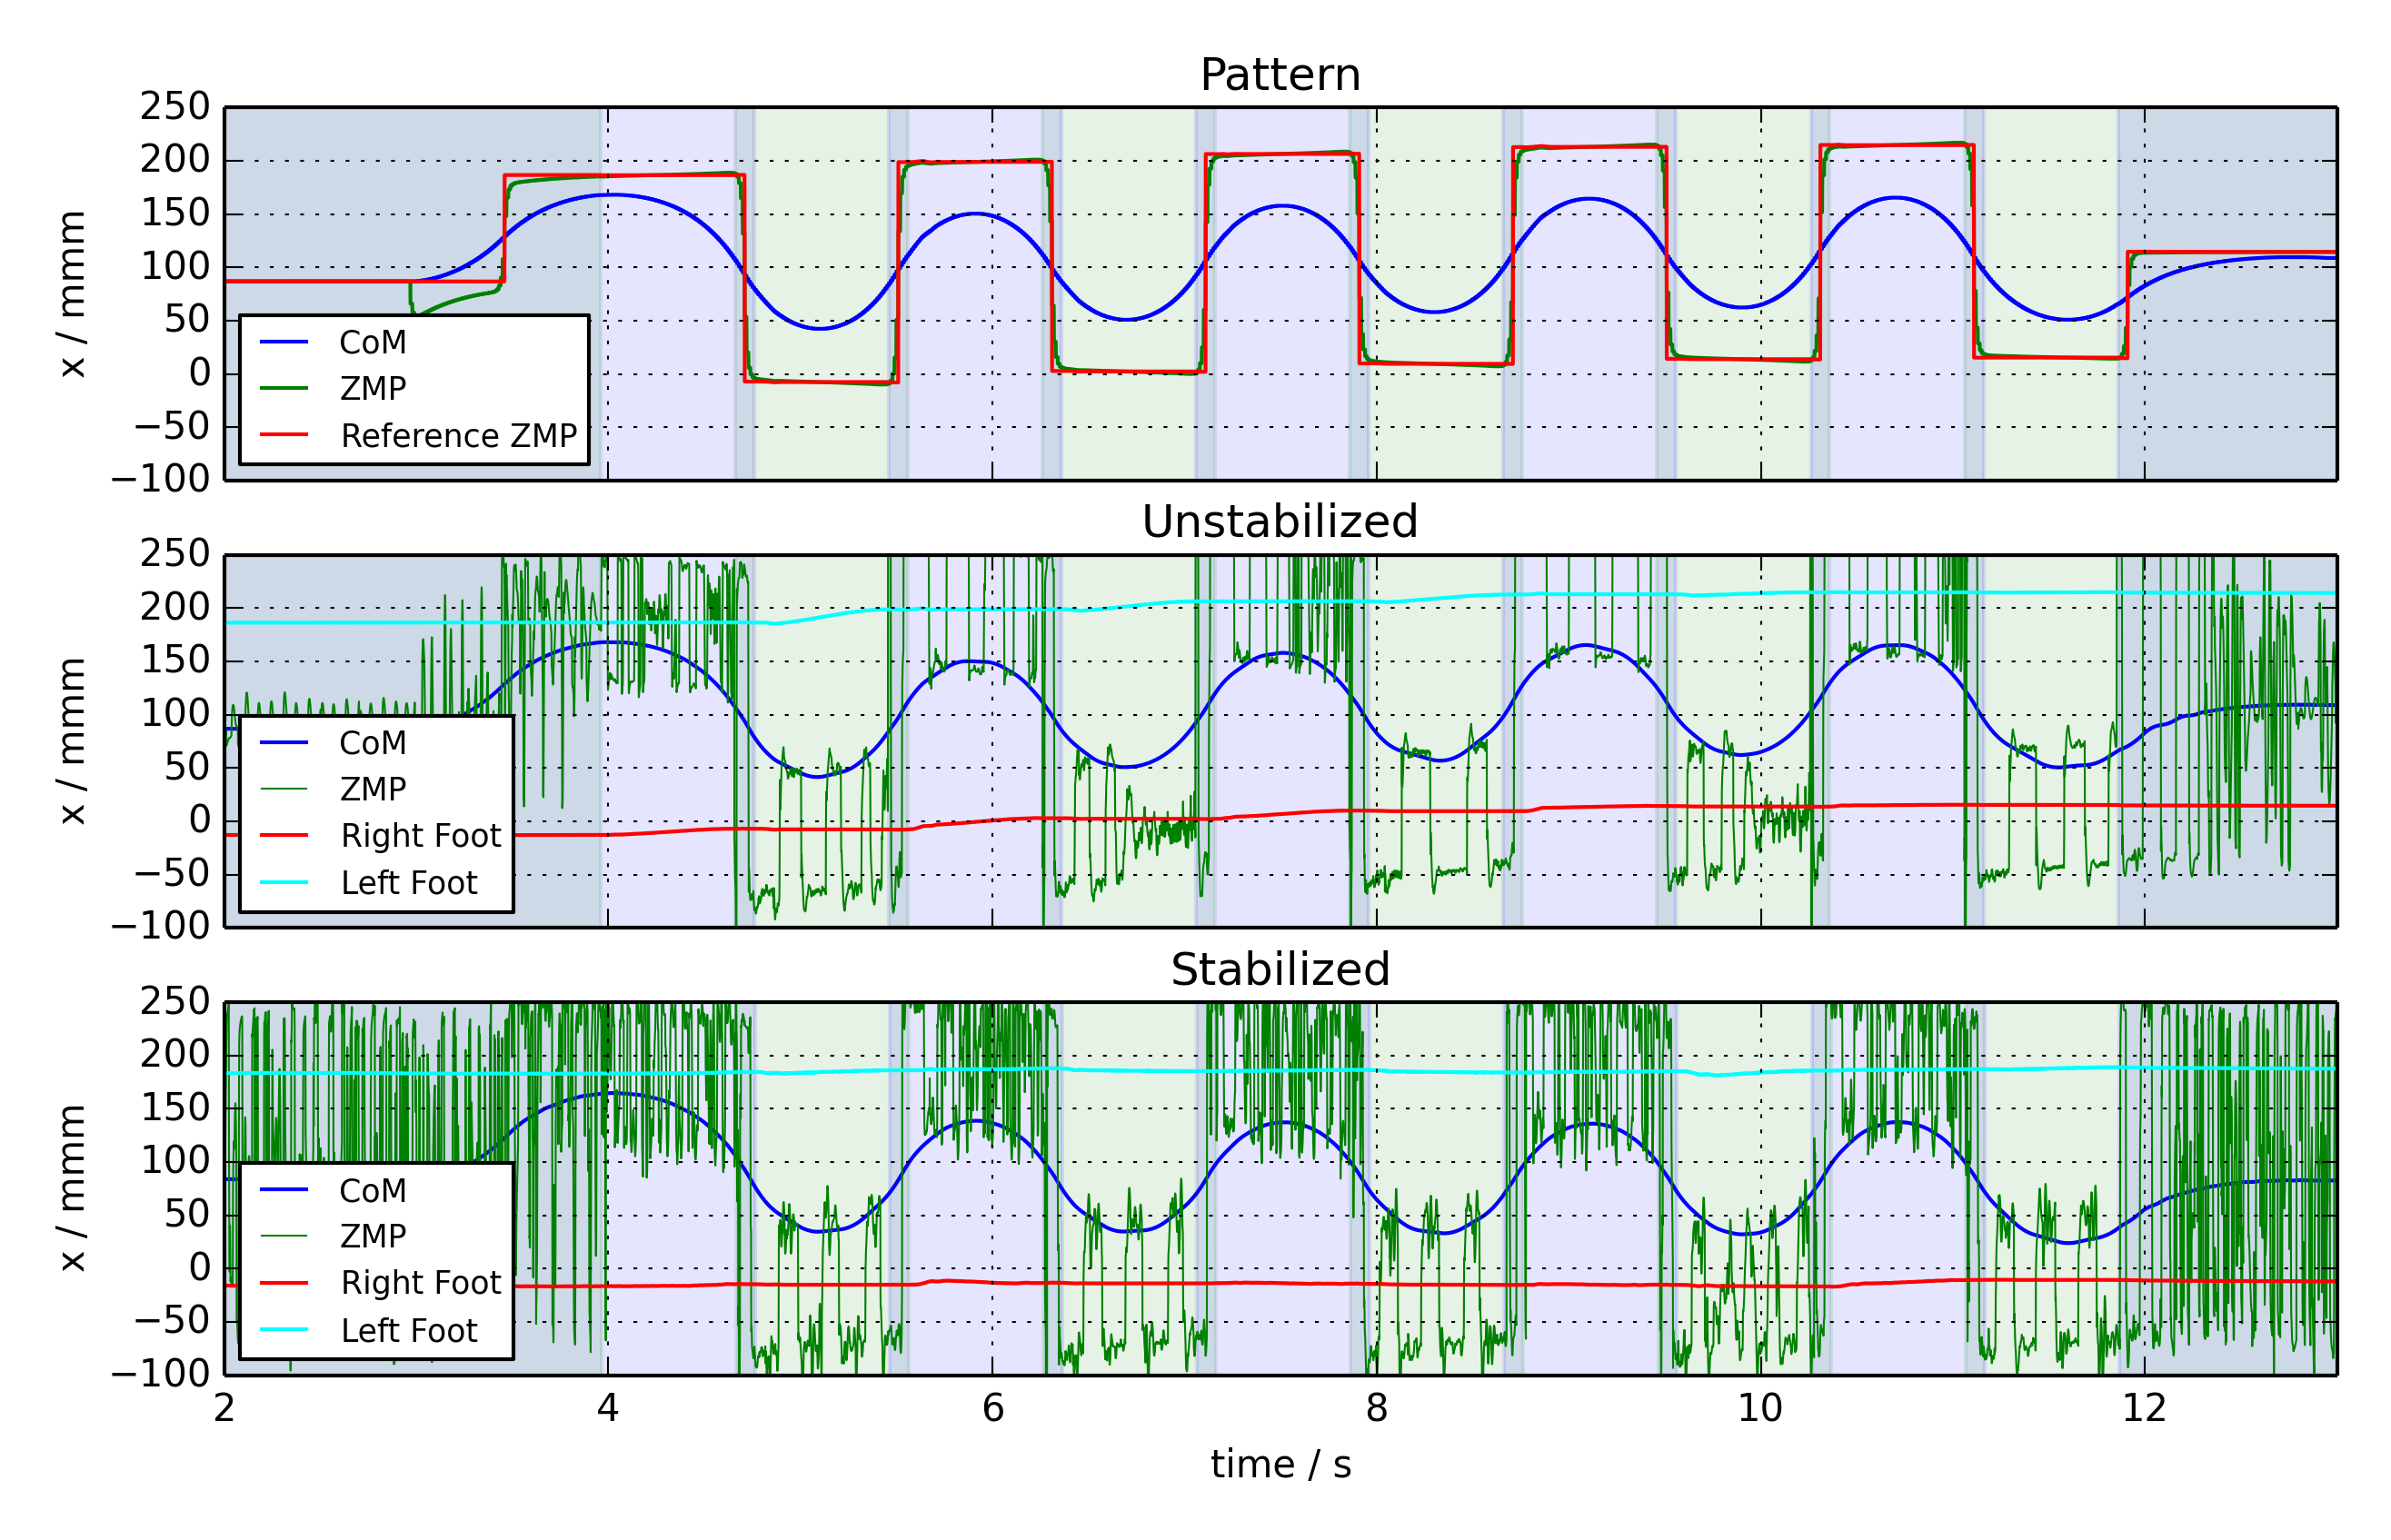
\includegraphics[width=\textwidth,resolution=300]{images/undisturbed_straight_x.png}
\caption{CoM and ZMP as specified by the pattern (top) and actual realized values (middle and bottom).
All coordinates in the global reference frame.}
\label{img:undisturbed-straight-x}
\end{figure}

Figure \ref{img:undisturbed-straight-x} shows the desired and realized
CoM and ZMP trajectories in both cases. As you can see the ZMP deviates
significantly from the desired trajectory and oscillates between both
edges of the support polygon. We believe this is caused by the problems
outlined in section \ref{section:rigid-body-simulation}. Consider figure
\ref{img:noisy-com-acc} which shows the desired CoM acceleration in
comparison to the realized acceleration. However the foot remains in
full ground contact and friction forces are applied accurately. Thus
dynamically stable walking is realized for both unstabilized and
stabilized walking. We hope that a more stable Featherstone constraint
solver will produce more accurate contact forces and thus ZMP values.

\begin{figure*}[hbt]
\vspace*{-1em}
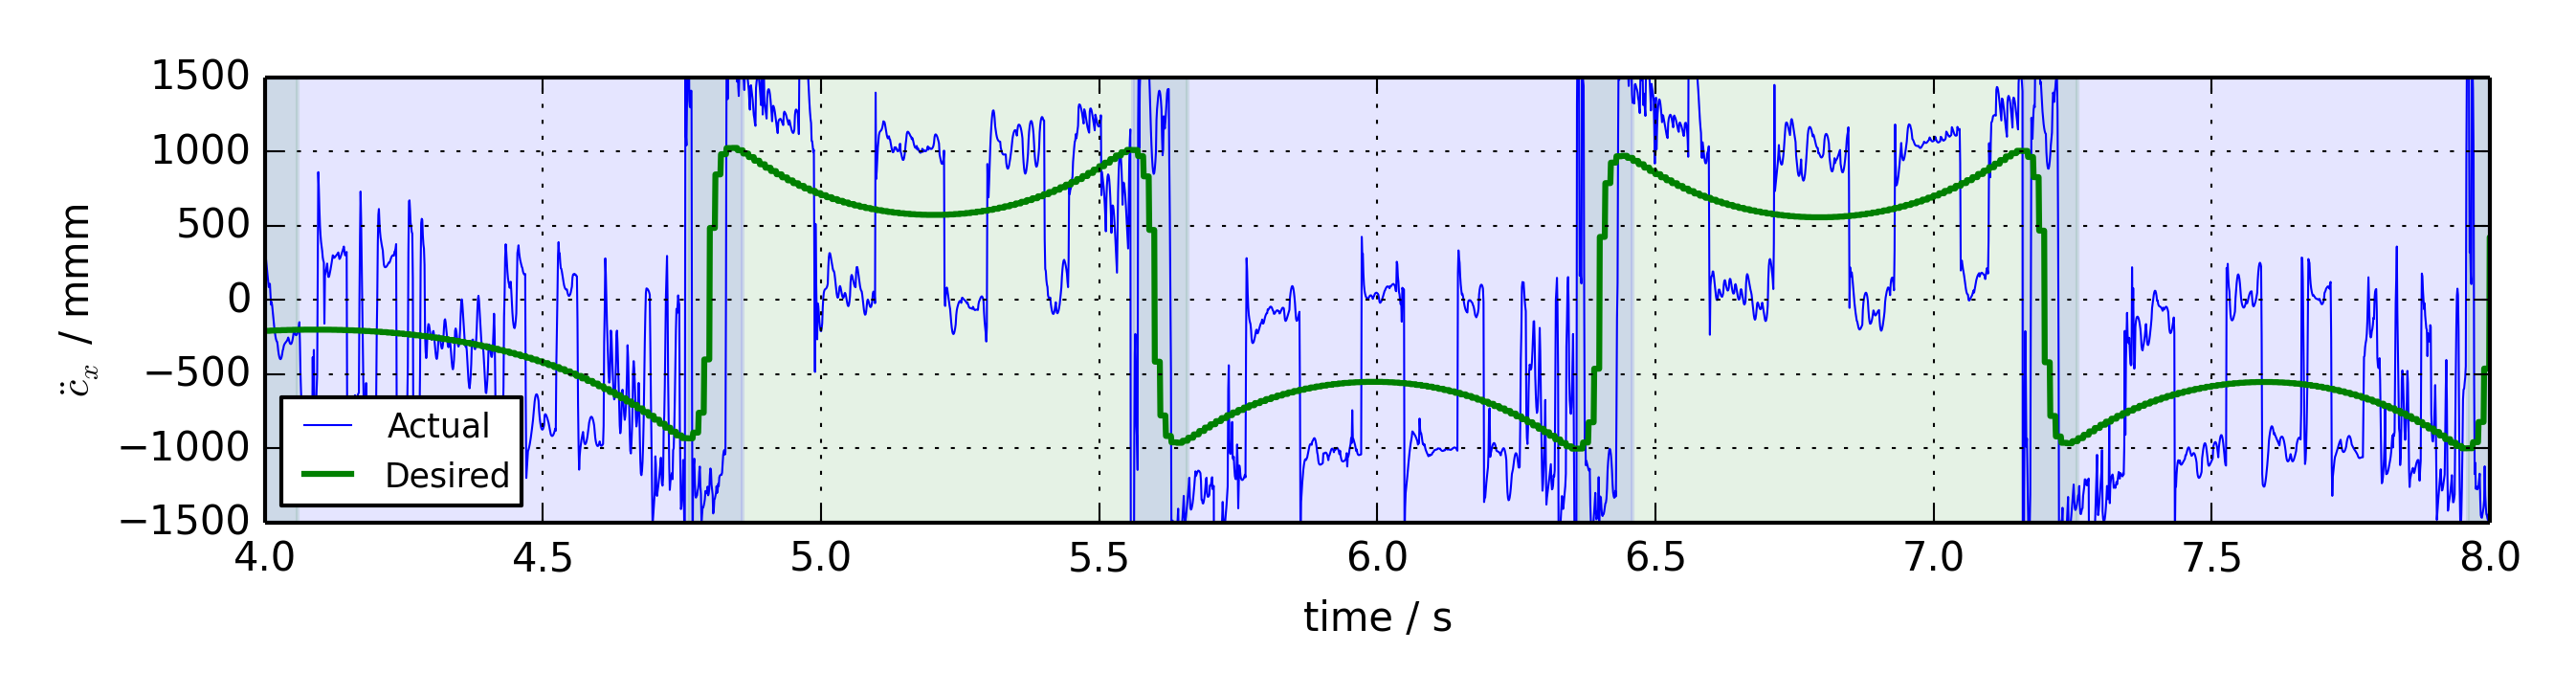
\includegraphics[width=\textwidth,resolution=300]{images/noisy_com_acc.png}
\caption{Acceleration of the CoM in $x$-direction.}
\label{img:noisy-com-acc}
\end{figure*}

\subsection{Walking in a circle}\label{walking-in-a-circle}

\begin{figure*}[hbt]
\vspace*{-1em}
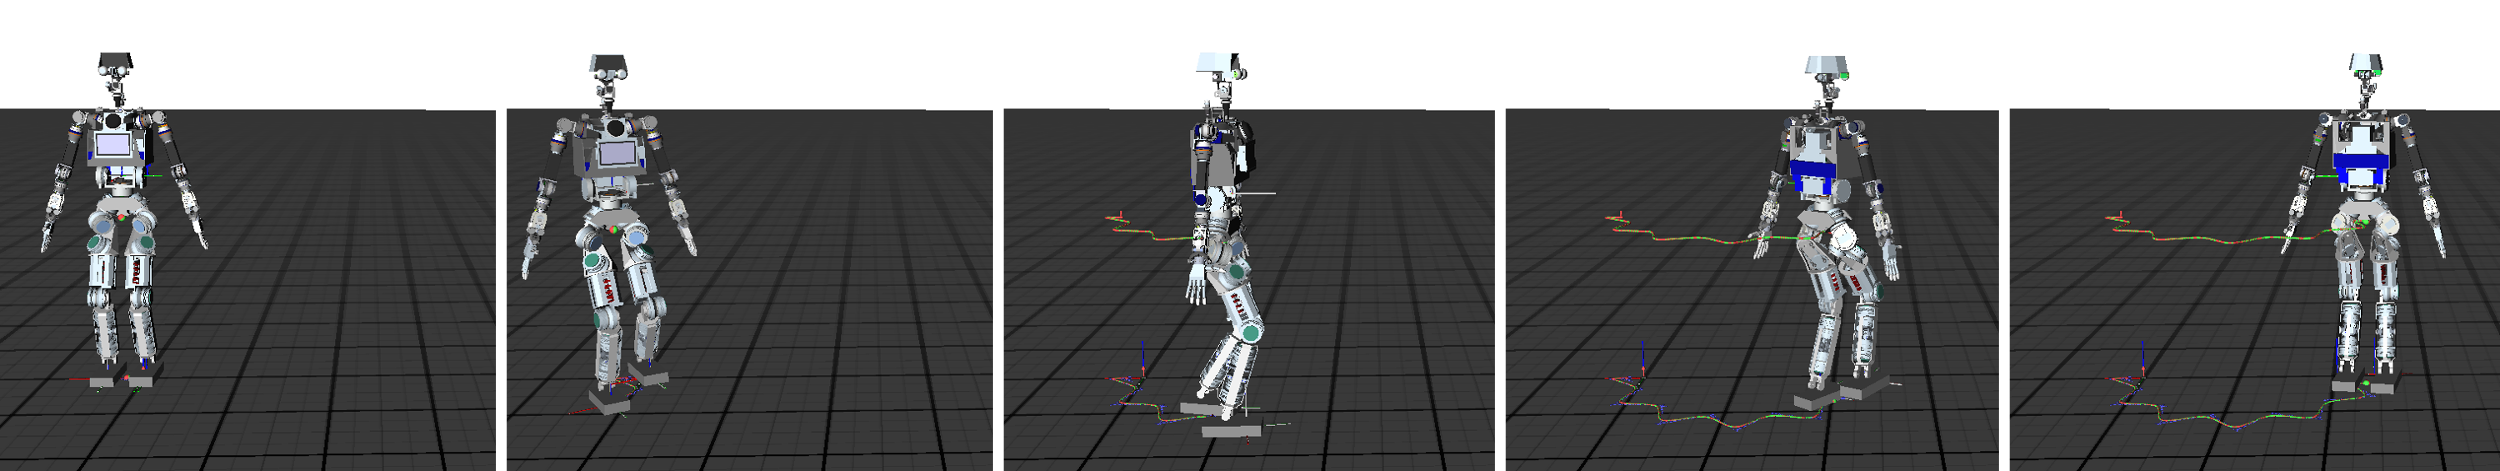
\includegraphics[width=\textwidth,resolution=300]{images/undisturbed_circle_thumbs.png}
\caption{\name{Armar4} walking in a half circle in 12 steps.}
\label{img:player-undisturbed-circle-thumbs}
\end{figure*}

Figure \ref{img:player-undisturbed-circle-thumbs} shows the simulation
of unstabilized walking in a circle. The robot walks in 12 steps in an
arc of 180° and 0.5 m radius. As you can see the desired 180° turn is
not realized completely. Due to the chest rotation following the tangent
of the circle, a torque around the yaw-axis is exerted on the foot.
Recall that during pattern generation we assumed that this torque is
zero. Since we do not correct this disturbance the trajectory deviates
significantly. See figure \ref{img:undisturbed-circle} for the realized
ZMP distribution and CoM trajectory for both unstabilized and stabilized
walking. The unstabilized trajectory will get unstable towards the end
of the trajectory. However the stabilized trajectory remains stable.

\begin{figure}[hbt]
\vspace*{-1em}
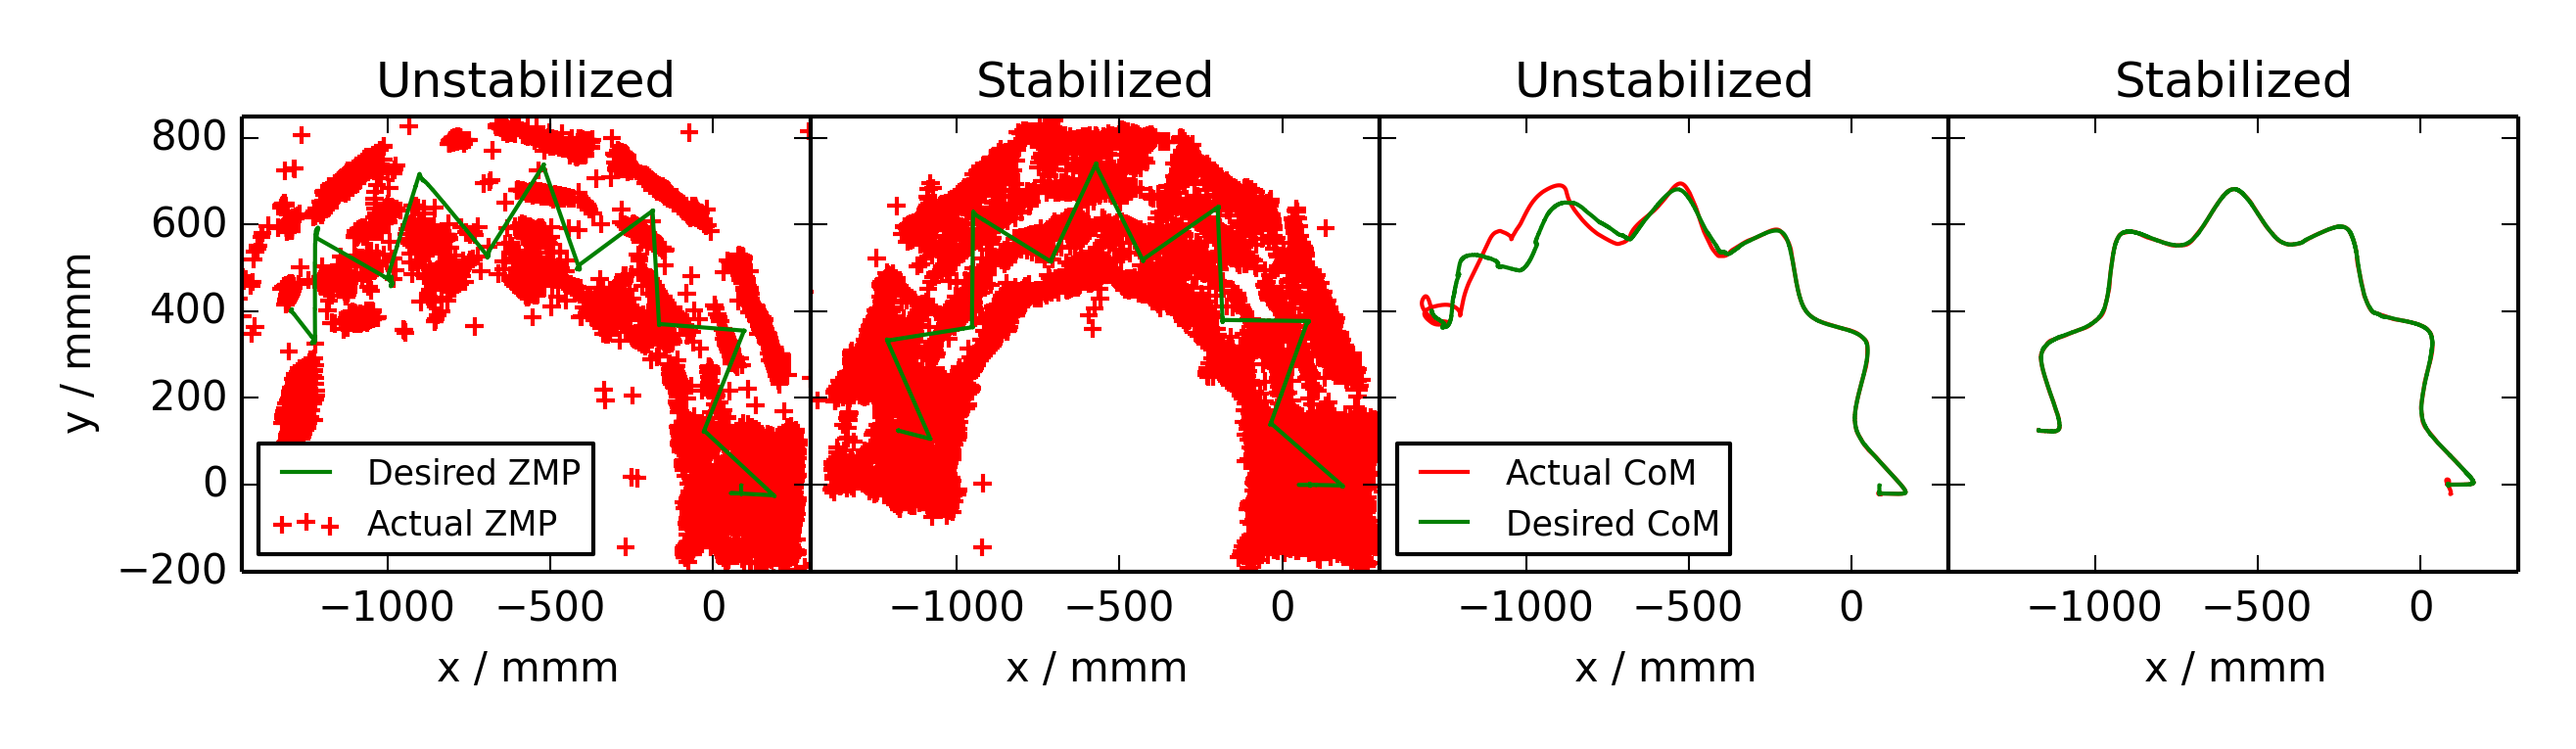
\includegraphics[width=\textwidth,resolution=300]{images/undisturbed_circle.png}
\caption{Walking in a cricle. ZMP (left) and CoM (right) as specified by the pattern and the actually realized values.
Each for the unstabilized and stabilized case.}
\label{img:undisturbed-circle}
\end{figure}

\section{Disturbed walking}\label{disturbed-walking}

The scenario used to test the performance of the stabilizer under
disturbance, was applying a short push to the chest. The results are
compared with the performance of the unstabilized trajectory.

\begin{figure*}[hbt]
\vspace*{-1em}
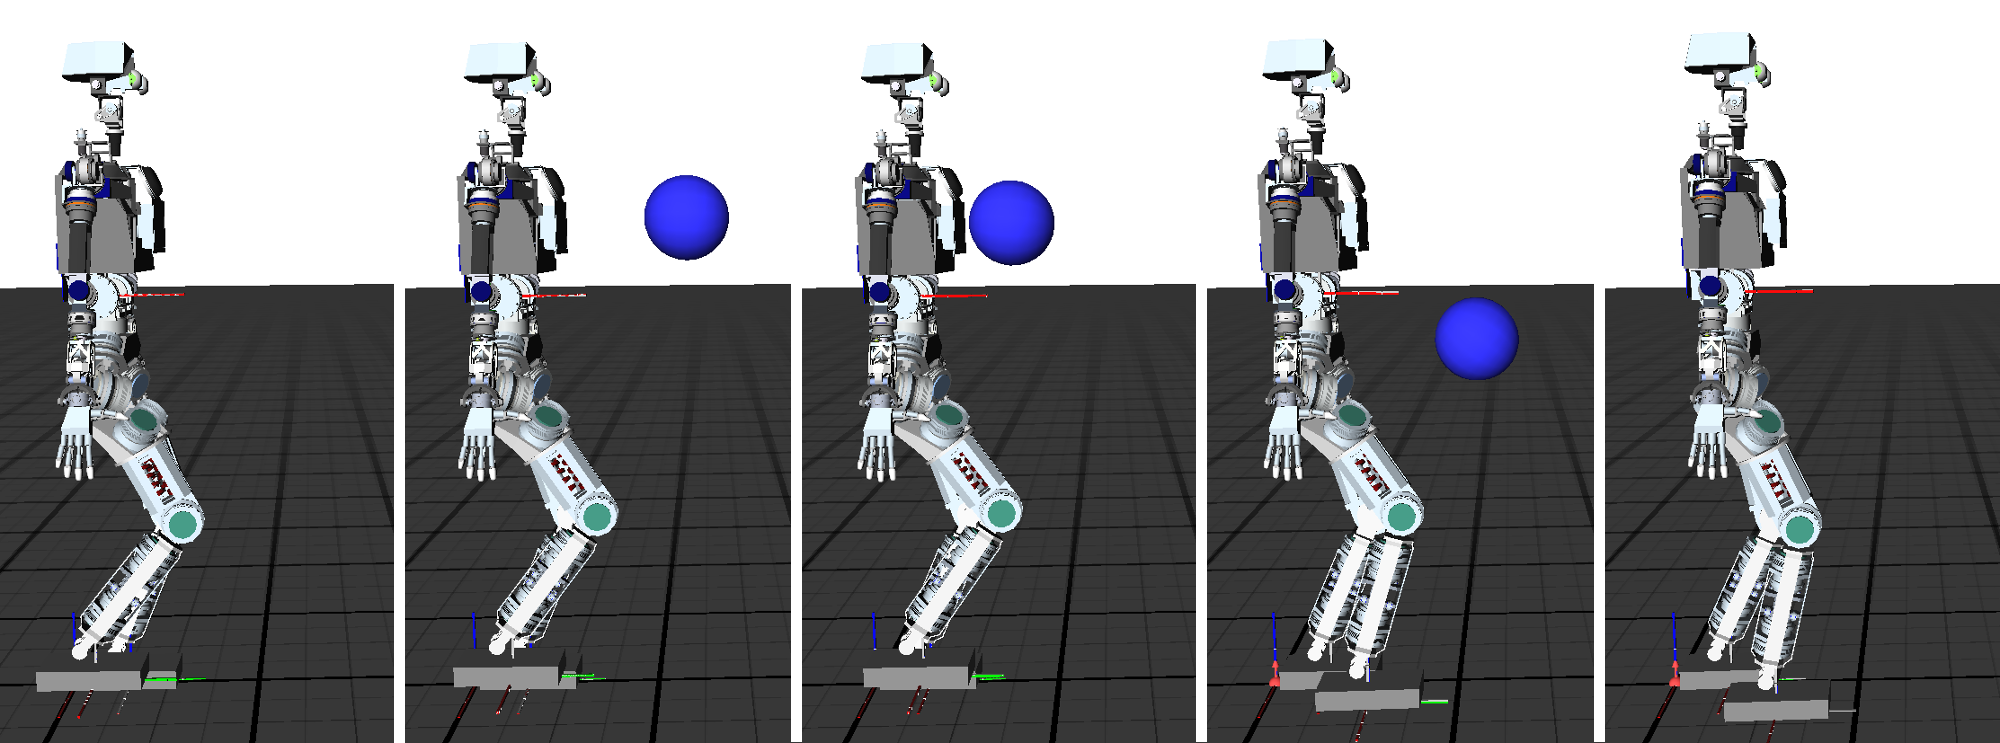
\includegraphics[width=\textwidth,resolution=300]{images/disturbed_straight_thumbs.png}
\caption{\name{Armar4} getting hit by a ball at chest height.}
\label{img:player-undisturbed-circle-thumbs}
\end{figure*}

To simulate a push, a ball with a radius of 11cm and weight of 450g
(FIFA football) is shoot from 1 meter distance at the chest. See figure
\ref{img:disturbed-straight-x} for the realized CoM and ZMP
trajectories. The point of impact is denoted as red lines. The
unstabilized trajectory becomes unstable and leads to a fall at
$t = 9.5s$. The stabilized trajectory is noticeable disturbed, as the
yaw momentum is not compensated, but remains stable.

\begin{figure*}[hbt]
\vspace*{-1em}
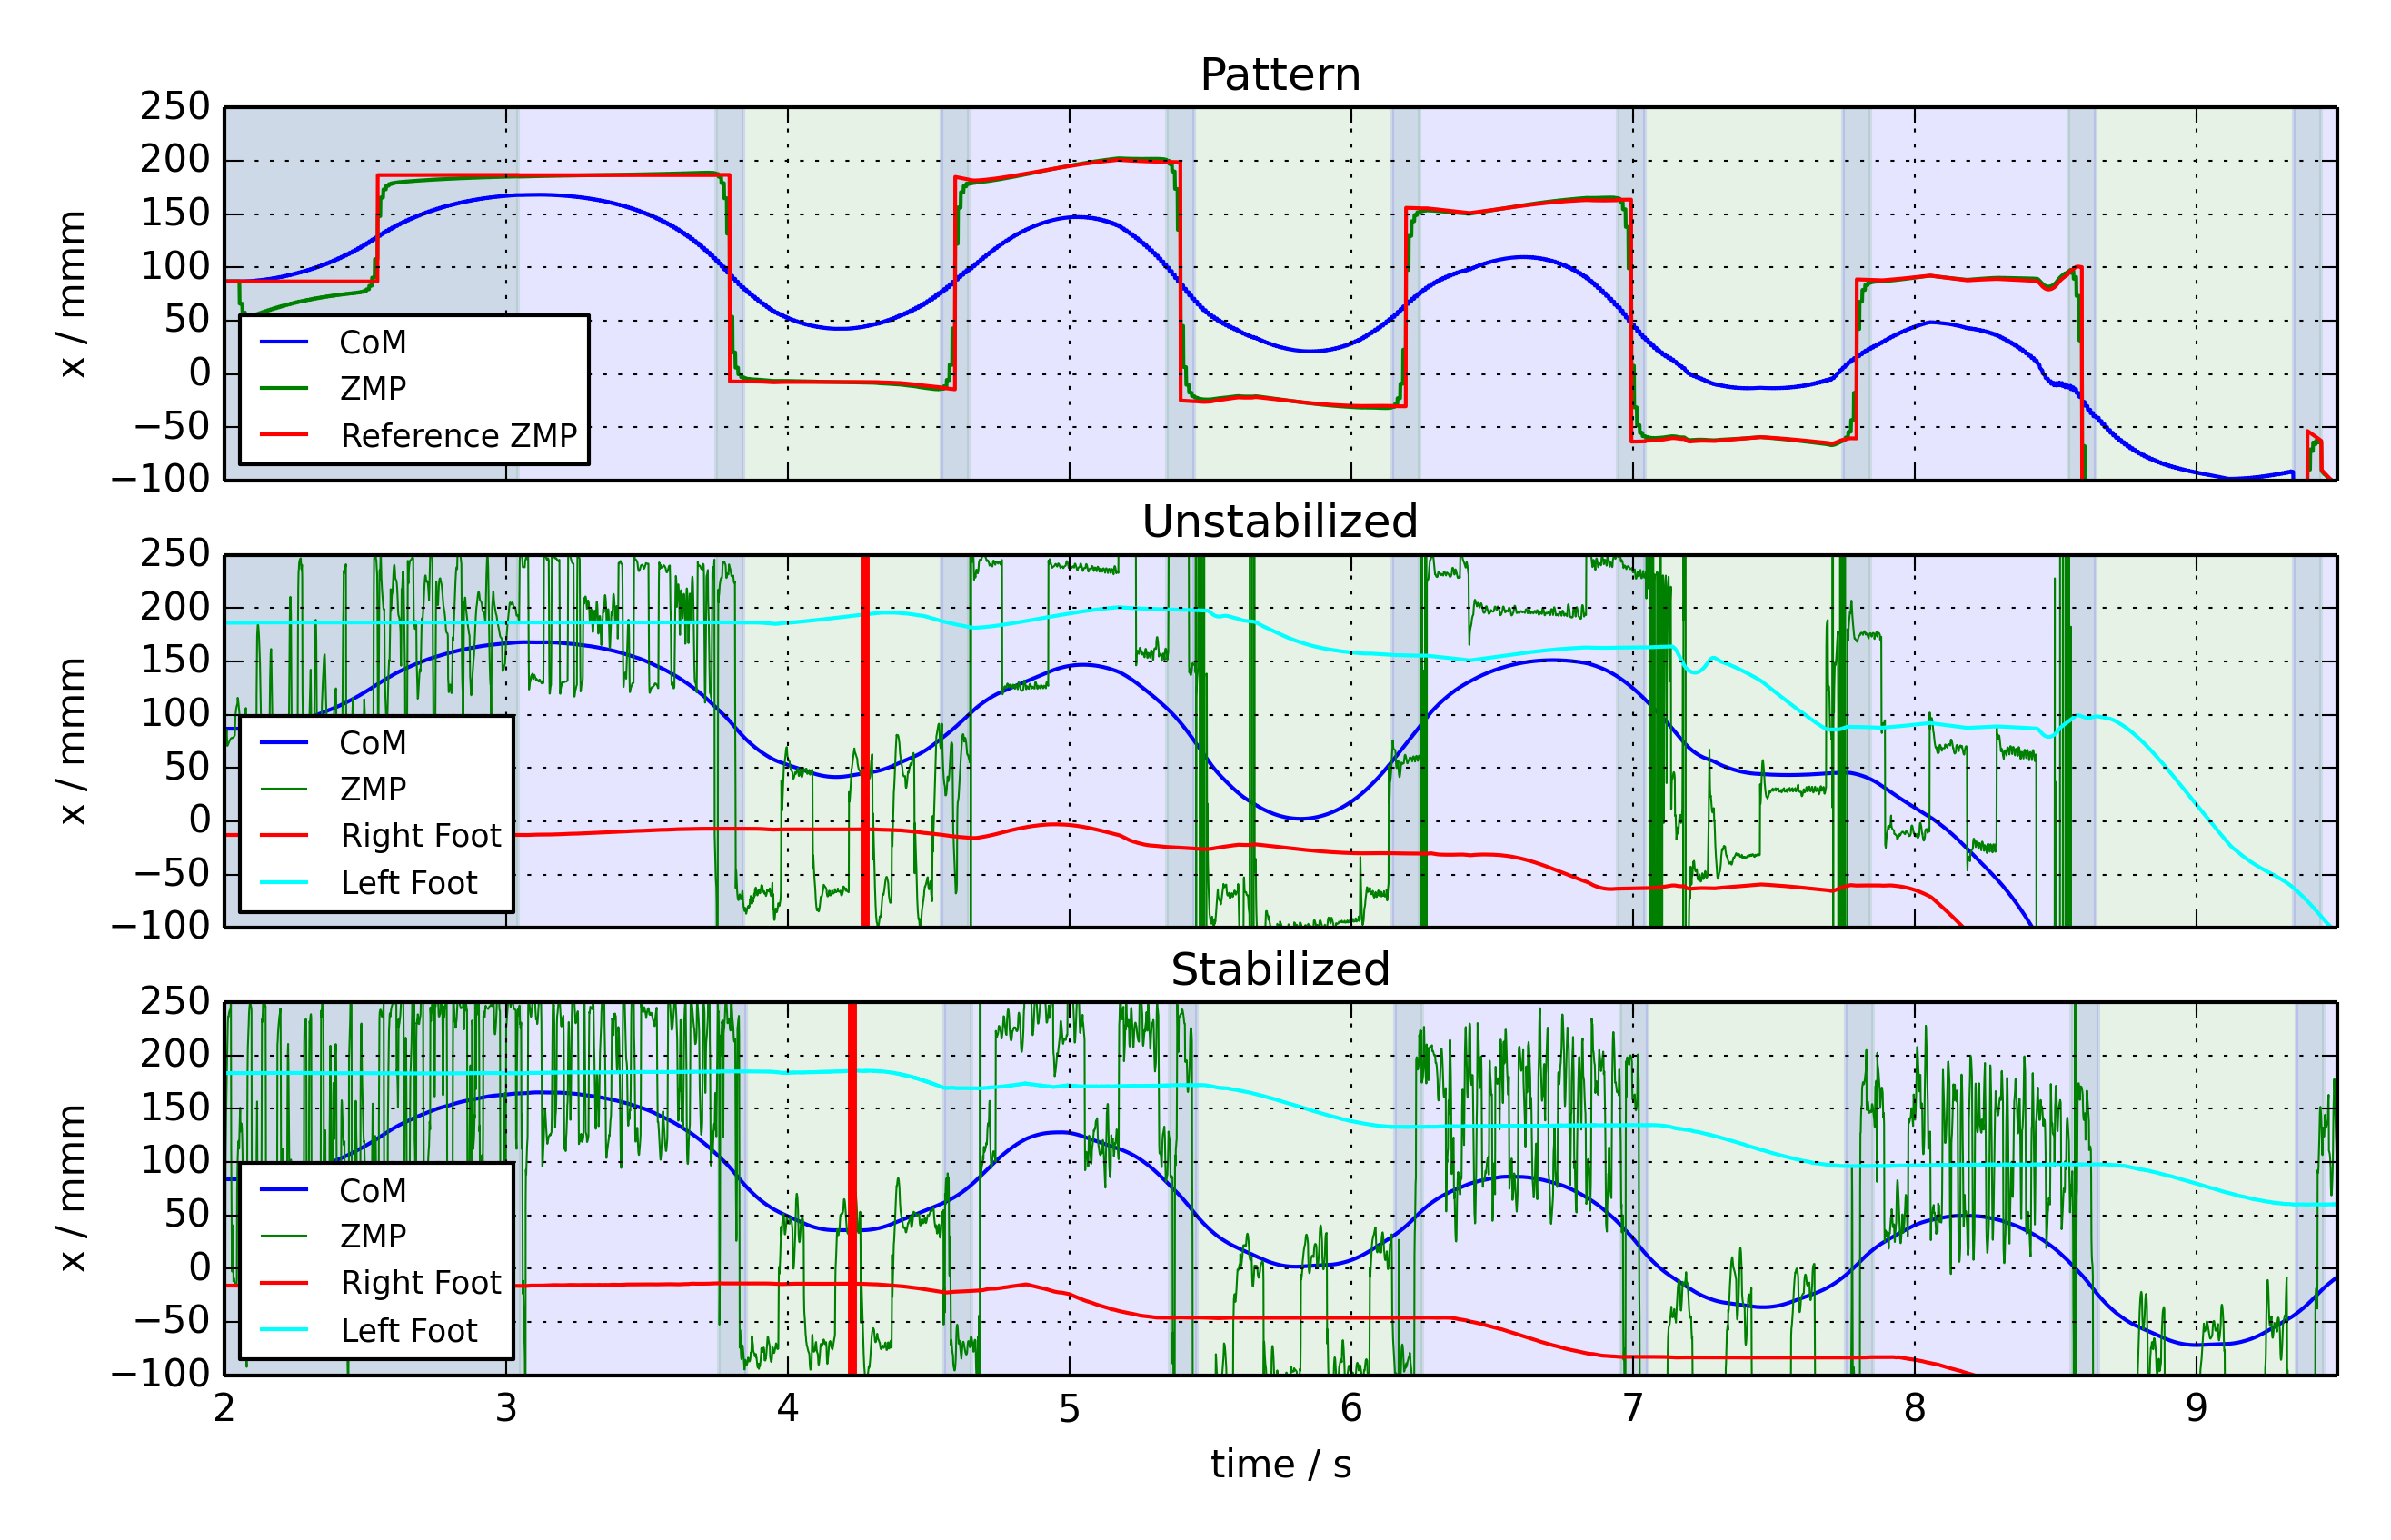
\includegraphics[width=\textwidth,resolution=300]{images/disturbed_straight_x.png}
\caption{CoM and ZMP as specified by the pattern (top) and actual realized values (middle and bottom).
All coordinates in the global reference frame. Red lines denote the point of impact.}
\label{img:disturbed-straight-x}
\end{figure*}

\section{Push recovery}\label{push-recovery-1}

The performance of the push recovery was evaluated with a simple
best-case scenario. The robot is balancing on the left foot and is
pushed on the right shoulder. Most notably this scenario was used to
demonstrate the push recovery based on the Capture Point implemented in
the IHMC/Yobotics Biped. \cite{pratt2009video}. While the push recovery
implemented is able to recover from any position, with the current
method it is not reliable in the general case. This has multiple reason,
for one the fall detection is not very reliable. Another reason is that
the speed limits of the leg joints impose a maximum velocity for the
foot movement. So not only needs the target position to be reachable, it
also needs to be reachable in a specific amount of time. As above a
football is used as source of disturbance. See figure
\ref{push-recovery-thumbs} for a push recovery.

\begin{figure*}[hbt]
\vspace*{-1em}
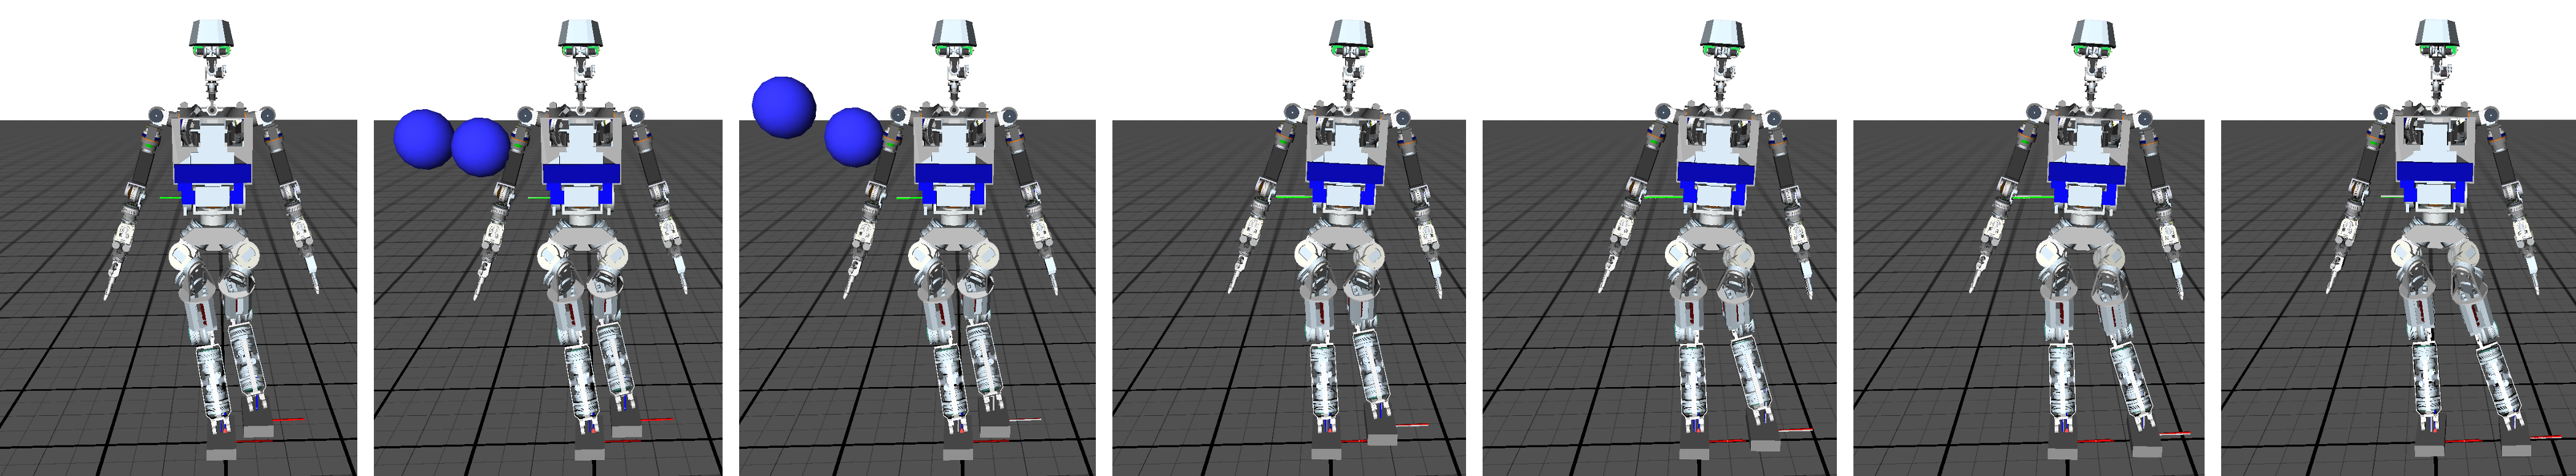
\includegraphics[width=\textwidth,resolution=300]{images/push_recovery_thumbs.png}
\caption{\name{Armar4} getting hit by two balls at the left shoulder.}
\label{img:push-recovery-thumbs}
\end{figure*}

\chapter{Conclusion and future work}\label{conclusion-and-future-work}

A design and the implementation of a software framework for bipedal
humanoid walking were presented. Building on an implementation by Ömer
Telemz, a generator for walking pattern using ZMP Preview Control was
developed. To test the resulting patterns a dynamic simulation for
walking was build. The simulation utilizes the \name{SimDynamics}
framework contained in \name{Simox}. The simulation was extended by
real-time controllers for stabilization and push recovery. For easily
integration into other software projects all methods presented here are
implemented in a shared library \name{libBipedal}. \name{libBipedal} is
independent of the dynamic simulation and only depends on
\name{VirtualRobot} for computing forward and inverse kinematics.

Evaluation showed that stable walking could be realized in simulation.
By applying a stabilizer the trajectories remained stable, even when
faced with disturbances. Falling was avoided by initiating a push
recovery mechanism based on the Capture Point.

Since accuracy of the dynamic simulation suffered severely by using the
Sequential Impulse Solver method, it should be replaced by a solver
based on the Featherstone method. The improved accuracy should make a
torque feedback more viable and enable to actually use the stabilizer
based described and implemented in \ref{section:stabilizer}.

The pattern generator and stabilizer only realize basic walking, that is
noticeable different to human walking. For one the knees remain bent at
all times, the center of mass stays at the same height and the toe joint
is not used. A follow up paper \cite{kajita2012evaluation} extends the
methods implemented here to include the toes. The realized walking
trajectories seem to be more natural.

As the evaluation of the circular trajectory shows, the yaw moment
exerted on the foot can cause severe disturbances. To deal better with
trajectories that include turns or arm movements, that torque should be
compensated. Kim et. al \cite{kim2005humanoid} propose to move the arms
around the roll axis to compensate for yaw momentum.

The push recovery implemented is very rudimentary. The placement of the
foot to recover from a push does not consider collisions with the
environment. Also, after executing a push recovery step, the original
trajectory can not be resumed. To enable that, online planning of
dynamically stable motions needs to be integrated. Also the foot is
placed at the exact location of the future capture point. However it
suffices to place the foot in a way to include the capture point. In
most cases this would requires a lot less foot movement. Moving the leg
to the target point also changes the velocity of the CoM, thus changes
the location of the capture point. To compensate this, the capture point
should be tracked using a controller instead of using a static future
capture point.

\bibliographystyle{ieeetr}

\bibliography{ba}

\end{document}
